\documentclass{ctexart}

\usepackage{graphicx}
\usepackage{subfigure}

\newcommand{\para}[1]{\noindent {\bf #1}}%remove \smallskip

\newcommand{\codeword}[1]{\texttt{\small{#1}}}

%%%%%%%%%%%%%%%%%%%%% BNF
\newcommand{\rulesep}{\unskip\ \vrule\ }
\newcommand \bnfdef  {\mathrel{\color{blue}{::=}}}
\newcommand \bnfalt  {\mathrel{\color{blue}{|}}}

\newcommand \keyfont {\mathsf}
\newcommand \ONPKT {\keyfont{onPacket(pkt)}}
\newcommand \WHILE  {\keyfont{while}}
\newcommand \IF     {\keyfont{if}}
\newcommand \THEN     {\keyfont{then}}
\newcommand \SKIP   {\keyfont{skip}}
\newcommand \RETURN   {\keyfont{return}}
\newcommand \ADD   {\keyfont{add}}
\newcommand \CONTAINS   {\keyfont{contains}}
\newcommand \GET   {\keyfont{get}}
\newcommand \PUT   {\keyfont{put}}
\newcommand \GLOBAL   {\keyfont{global}}
\newcommand \forl   {\keyfont{for}}
\newcommand \while[2]   {\WHILE\ {#1}\ {#2}}
\newcommand \ifelse[3]  {\IF\ {#1}:{#2}\ \THEN:{#3}}
\newcommand \return[1]   { \RETURN\ {#1}}
\newcommand \CYCLIC  {\keyfont{loop}}
\newcommand \cyclic[1]   { \CYCLIC\ {#1}}

\newcommand \JUMP  {\keyfont{jump}}
\newcommand \CJUMP  {\keyfont{cjump}}
\newcommand \LBL  {\keyfont{label}}

\newcommand \jump[1]   { \JUMP\ {#1}}
\newcommand \cjump[3]   { \CJUMP\ {#1}\ {#2}\ {#3}}
\newcommand \lbl[1]   { \LBL\ {#1}}

\newcommand \tx {\mathtt{x}}
\newcommand \ty {\mathtt{y}}
\newcommand \tz {\mathtt{z}}
\newcommand \tg {\mathtt{g}}
 
\begin{document}
 
\section{引言}

近年来SDN的成功~\cite{swan, b4, edgefabric} 促使研究人员考虑将其应用于军事联合(military coalition)中,以实现一个高效、敏捷的软件定义联合(Software Defined Coalition,SDC)~\cite{vinod-sdc}。在SDC网络中,多个联合成员可以在一个高动态并受限(如电力)的战术网络中进行操作。

%
%The recent success of software defined networking~(SDN) systems~\cite{swan, b4,
%edgefabric} motivates the efforts to integrating SDN into military coalitions to
%realize an efficient, agile, and optimal software-defined coalition (SDC)
%infrastructure~\cite{vinod-sdc}. In SDC, autonomous coalition members operate
%under highly dynamic tactical network environments with resource constraints,
%such as limited power and processing capability, and dynamic connectivity. 

将SDN与军事联合结合并形成SDC的想法相对直观,因为通过SDN数据面上的灵活的数据包匹配处理和控制面上的集中式控制,联合成员可以在联合网络上实现高效、灵活的控制~\cite{p4, rmt}。然而这些突出的性质仍然无法充分满足需求。

%One may think that the integration of SDN into SDC is straightforward, because SDN
%allows coalition members to realize efficient, flexible control over the
%coalition networks through flexible packet match-action processing on the data
%plane and logically centralized in the control plane~\cite{p4, rmt}.
%Despite these promising features, they are insufficient for supporting SDC.

根本原因是在一个高动态战术网络环境中,SDC应用(例如灵活的负载均衡、DNS放大攻击的探测)对性能(例如实时性、高效性、可靠性)有着非常苛刻的要求。在一个高动态战术网络环境中通过传统SDN架构运行的SDC应用,由于数据面和控制面之间频繁的数据传输,会受到严重的时延等问题。

%The fundamental reason behind this insufficiency is that SDC applications (\eg,
%flexible load-balancing and detection of DNS amplification attack) have
%stringent performance requirements (\eg, real-time, efficiency and reliability) 
%under \textit{highly dynamic tactical network environments}. Implementing SDC
%applications using the above SDN architecture in such environment would incur high communication overhead
%between the data and control planes of SDC applications, resulting in
%significant delay, efficiency and reliability issues.

最近研究人员提出了一些新的SDC数据平面设计~\cite{bianchi2014openstate, opensdc}。它们将对数据包进行的复杂有状态的操作(例如计数、流安全探测、拥塞控制)从控制平面卸载到数据平面,以提高SDC应用的性能。在这些系统中,不同的数据平面原语,如状态计数器、数据包缓存以及数据包网络中计算(in-network compute)模块被设计出来以支持不同的SDC应用,如有状态防火墙、主动路由保护、弹性路由等。

%Some SDC datapaths are recently proposed, which offload \textit{complex,
%stateful} operations on packets (\eg, counting, flow security inspection and
%congestion control) from the control plane to data plane
%devices to improve the performance of SDC
%applications~\cite{bianchi2014openstate, opensdc}.  Different datapath primitives, such as state
%counter, packet buffer and packet in-network processing block, are designed in
%these systems to support various SDC applications, \eg, stateful firewall,
%proactive routing protection, and resilient routing. 

然而,这些系统有以下两点不足:1. 那些被卸载到数据平面上的有状态操作的结果(以下我们称之为本地状态)并没有在多个数据平面设备上进行共享,导致SDC网络中的巨大的资源浪费。例如,由于防火墙中间盒的有限的处理速度,其在SDC网络中经常是一个瓶颈。当一个数据流通过防火墙被标志为安全非敏感数据后,其数据流的后续数据包应该沿着一个高可靠高带宽的路径进行转发,而不同再次经过该防火墙。然而,由于该数据流的安全状态只保存在该防火墙设备而非共享给其他设备,在不确定该数据流是否安全情况下,一个上流设备(例如,一个网关路由器)仍然需要将所有数据包转发到该防火墙;2. 尽管已有一些分布式更新原语提供了在多个数据面设备之间共享本地状态的能力~\cite{ddp},配置这些低层次的SDC数据面任然需要花费大量的时间而且非常容易出错。

%However, these systems
%suffer from two limitations. First, results of offloaded stateful operations at
%data plane devices, which we refer to as \textit{local state} in the remaining
%of the paper, are not shared between data plane devices, resulting in
%substantial resource under-utilization in SDC networks. For example, a firewall
%middlebox is usually a bottleneck in an SDC network due to its
%limited processing speed. As such, once a data
%flow is identified as secure, non-sensitive by a firewall, all future packets of
%this flow should be forwarded along a path with higher reliability and throughput, without the need
%of passing the firewall again. However, the security state of this flow is only
%stored in the firewall and not shared with other devices. 
%Without knowing that this flow is non-malicious, an upstream
%device (\eg, a gateway router) in the SDC network still has to forward all the
%packets of this flow to the firewall. Second, although some distributed
%update primitives provide interfaces for sharing of local state between data
%plane devices~\cite{ddp}, configuring such low-level SDC datapaths still
%requires time-consuming and error-prone manual efforts.

%%Civilian high-level datapath programming systems, such as SNAP~\cite{snap}, do not support
%%the sharing of local state between data plane devices. Though this may 
%%work in more reliable civilian environments (\eg, campus and enterprise networks), 
%%it can substantially hurt the performance of SDC in the highly-dynamic tactical environments.  

为了解决以上两点不足,我们设计了Dandelion,一个高级SDC编程系统。Dandelion提出了一系列的创新的编程原语,使用户可以灵活地制定SDC数据平面设备的操作。除此之外,为了将高级SDC程序转为高效的SDC数据面配置,我们采用了一个决策图的数据结构和一个高效的配置框架。转化后的配置允许SDC网络中的数据平面设备互相交换本地状态以达到SDC网络资源(例如,设备数据包处理以及设备之间数据传输能力)的高效利用。

%Toward addressing these two limitations, in this paper, we design \concept{}, a
%novel, high-level SDC programming system. Specifically,
%\concept{} introduces a series of novel programming primitives for users to
%model and specify the behavior of SDC data plane devices. In addition, we design
%a novel data structure called \textit{decision graph} and an efficient
%configuration framework to translate high-level SDC programs into
%efficient SDC datapath configurations. The translated configurations allow data
%plane devices in SDC to exchange local states with the goal of efficiently
%utilizing the resources in SDC networks (\eg, the packet processing capability
%of devices and the data transmitting capability between devices). We implement a prototype of \concept{} and demonstrate its efficiency and efficacy using experiments. Results show that with \concept{}, the total
%throughput can increase around two times higher than that of without
%\concept{}.
%
%The rest of this paper is organized as follows. Section~\ref{sec:motivation}
%discusses related work and gives an motivating example. 
% Section~\ref{sec:system} gives an overview of \concept{} and Section~\ref{sec:details}
% presents the details of how \concept{} translates a high-level SDC program into data plane configurations. We evaluate the
% performance of \concept{} in Section~\ref{sec:eval} before concluding the paper
% in Section~\ref{sec:conclusion}.
 
\section{相关工作以及研究动机}
\para{相关工作}:
近期一些SDN/SDC数据平面的工作被提出~\cite{arashloo2016snap, heorhiadi2016simplifying, soule2014merlin, benet2018mp, katta2016hula, gember2012stratos, anwer2015programming, monsanto2012compiler, kohler2018p4cep, bianchi2014openstate, opensdc},它们主要的思想是将对数据包进行复杂有状态的操作(例如,计数、流安全探测、拥塞控制)从控制平面(例如,基站)卸载到数据平面设备(例如,移动设备)上,从而提高在动态战术环境中SDN应用的性能。在这些设计中,被卸载的对数据包操作的结果独立地存储在每个数据平面设备上。SOL~\cite{heorhiadi2016simplifying}和Merlin~\cite{soule2014merlin}在受限的网络状态环境下,通过计算路径,来解决数据平面设备的放置以及配置问题。P4CEP~\cite{kohler2018p4cep}和OpenSDC~\cite{opensdc}考虑拓展数据平面的能力,从可以进行简单的数据包处理到可以进行事件处理。SNAP~\cite{arashloo2016snap}设计一个高级网络编程系统,从而将一个高级程序转为有状态数据平面设备的配置。我们可以看出,尽管以上主要工作均关注SDC数据平面的设计,但这些系统的一个共同的限制是数据平面设备的本地状态无法共享给其他设备。下面的一个例子显示在SDC网络中这种情况会导致资源的不充分利用,进而影响SDC应用的性能。
 
%Some SDN/SDC datapaths are recently proposed to offload complex,
%stateful operations on packets (\eg, counting, flow security inspection and
%congestion control) from the control plane (\eg, a base station) to data plane
%devices (\eg, mobile devices) to improve the performance of SDN
%applications~\cite{arashloo2016snap, heorhiadi2016simplifying, soule2014merlin,
%benet2018mp, katta2016hula, gember2012stratos, anwer2015programming,
%monsanto2012compiler,
%kohler2018p4cep, bianchi2014openstate, opensdc} under dynamic
%tactical environments. 
%In these designs, results of offloaded operations are
%stored by each data plane device independently. We refer to them as
%\textit{local states}.
%SOL~\cite{heorhiadi2016simplifying} and Merlin~\cite{soule2014merlin}
%tackle the placement and configuration of data plane devices by solving
%constrained path computation problems.
%  P4CEP~\cite{kohler2018p4cep} and OpenSDC~\cite{opensdc} focus on expanding the
%capability of data plane devices from packet processing to event processing.
%SNAP~\cite{arashloo2016snap} designs a high-level programming system that
%translates a high-level program to the configuration of
%stateful operations in data plane devices. Despite these substantial efforts
%on stateful SDC datapath, one major, common limitation of these systems is that the local states of each data plane device are not
%shared with others. As we will show shortly in the motivating example, this would lead to
%substantial resource under-utilization in SDC networks, impairing the
%performance of SDC applications. 

为了允许在数据平面设备之间共享本地状态,DDP~\cite{ddp}对于分布式数据平面更新设计了一些原语。Hula~\cite{katta2016hula}和MP-HULA~\cite{benet2018mp}考虑的场景是数据平面设备上的负载均衡应用,并设计了一个发送以及接受探测数据包的机制以更新设备设备上的本地状态。然而,这些系统均需要用户根据不同应用手工地配置数据平面低级的原语,从而花费大量的时间并非常容易出错。

%To allow local state sharing between data plane devices, DDP~\cite{ddp} designs
%some  primitives for distributed datapath update. Hula~\cite{katta2016hula} and
%MP-HULA~\cite{benet2018mp} also design probing mechanisms for data plane devices
%running load balancing applications to update their local states.  However,
%manually configuring such low-level primitives on an application-by-application
%basis is time-consuming and error-prone.

\begin{figure}[!htbp]
%\vspace{-2mm}
\centering
\subfigure[\label{fig:fw-topo} 网络拓扑。]{
      \centering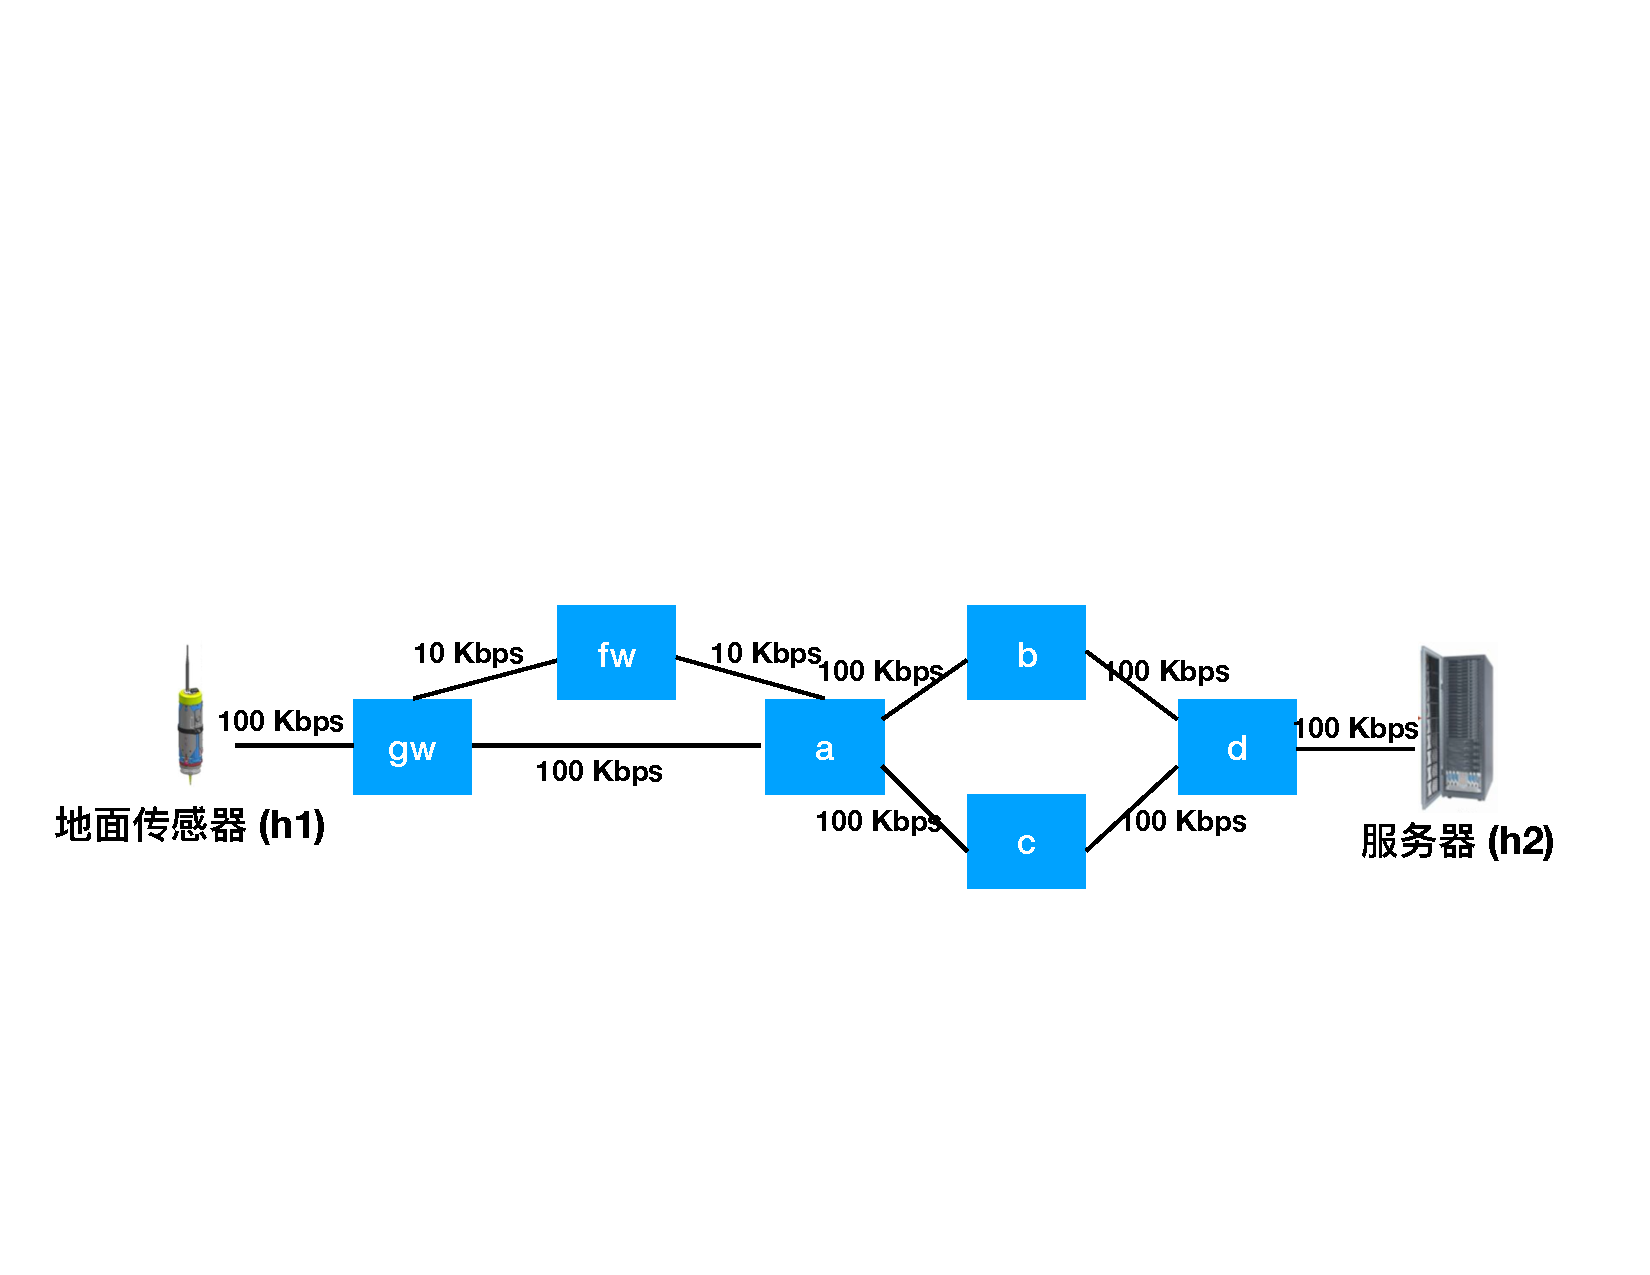
\includegraphics[width=\linewidth]{figures/ss-122.pdf}}
\hspace{0.03\linewidth}
\subfigure[\label{fig:existing-result}没有本地状态共享下的数据平面配置。]{
      \centering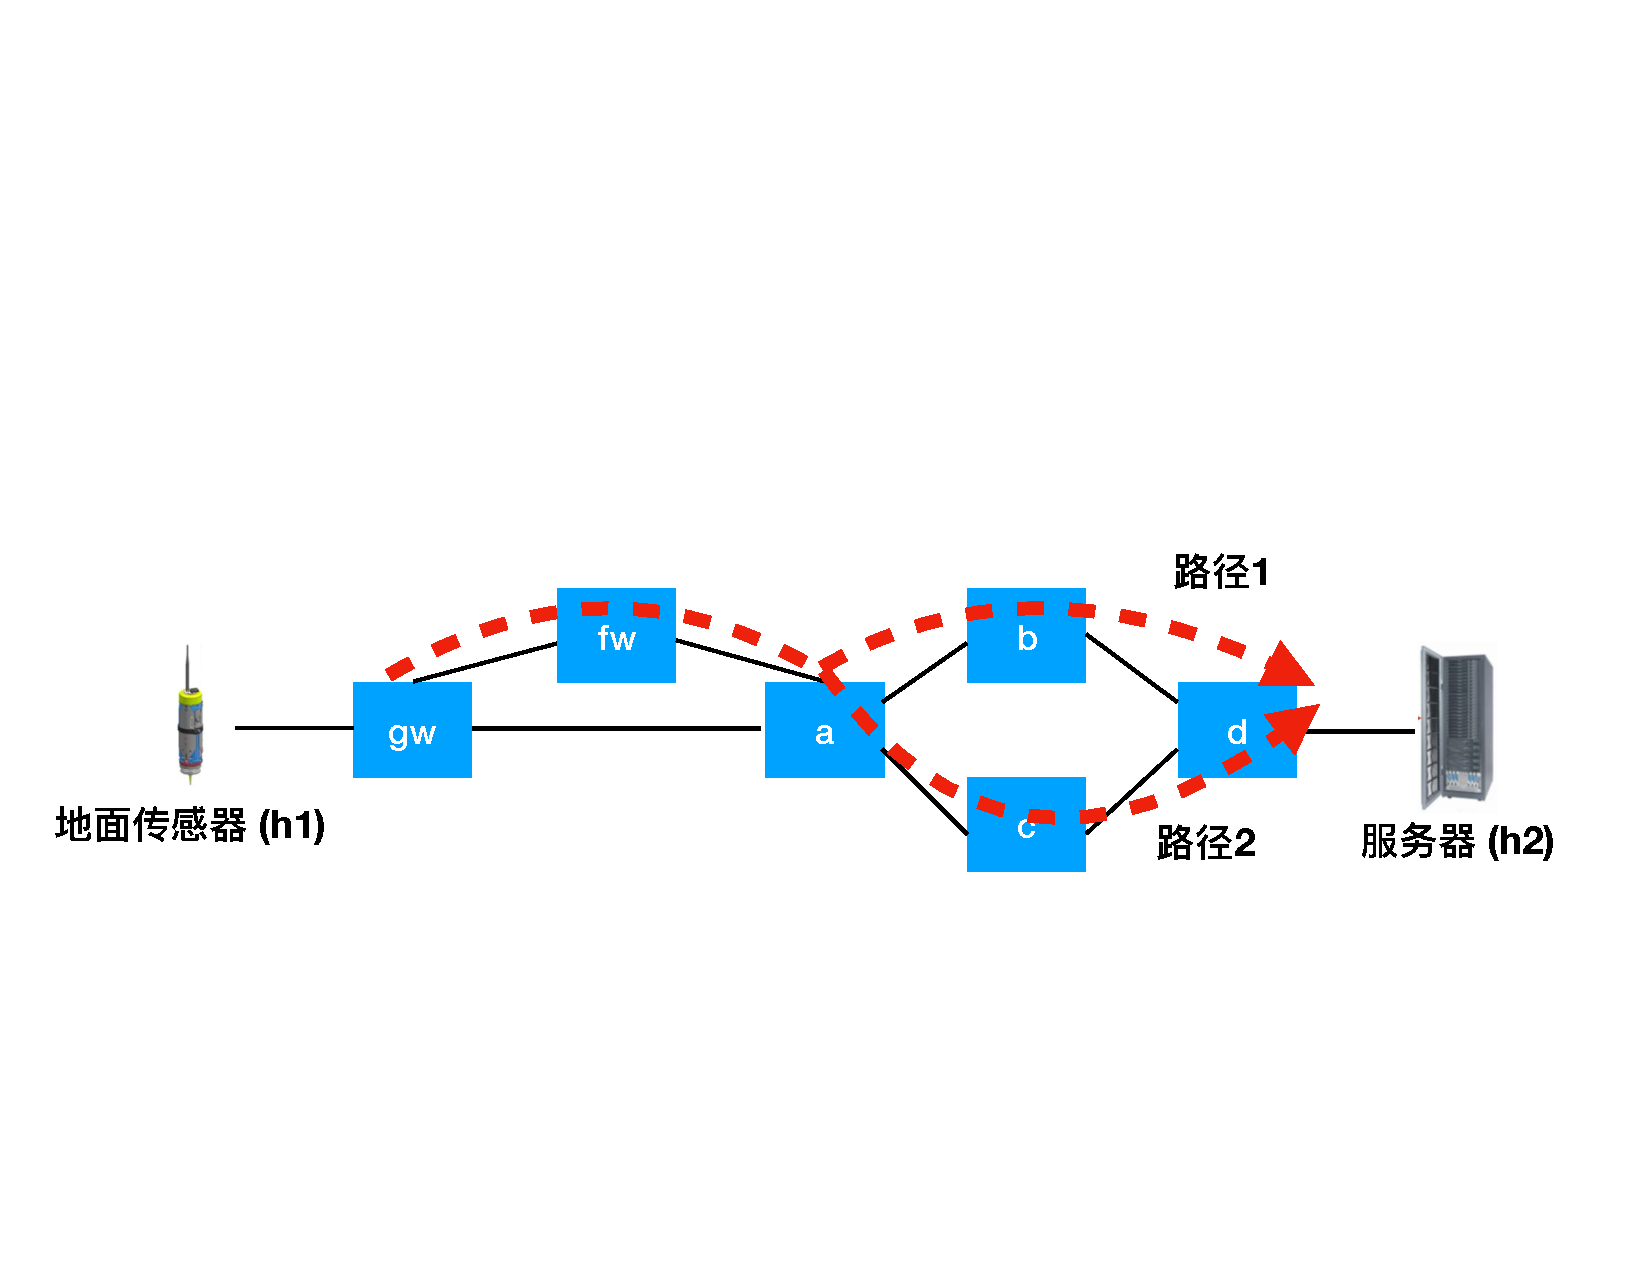
\includegraphics[width=\linewidth]{figures/ss-123.pdf}}
%\begin{subfigure}{0.8\linewidth}
%      \centering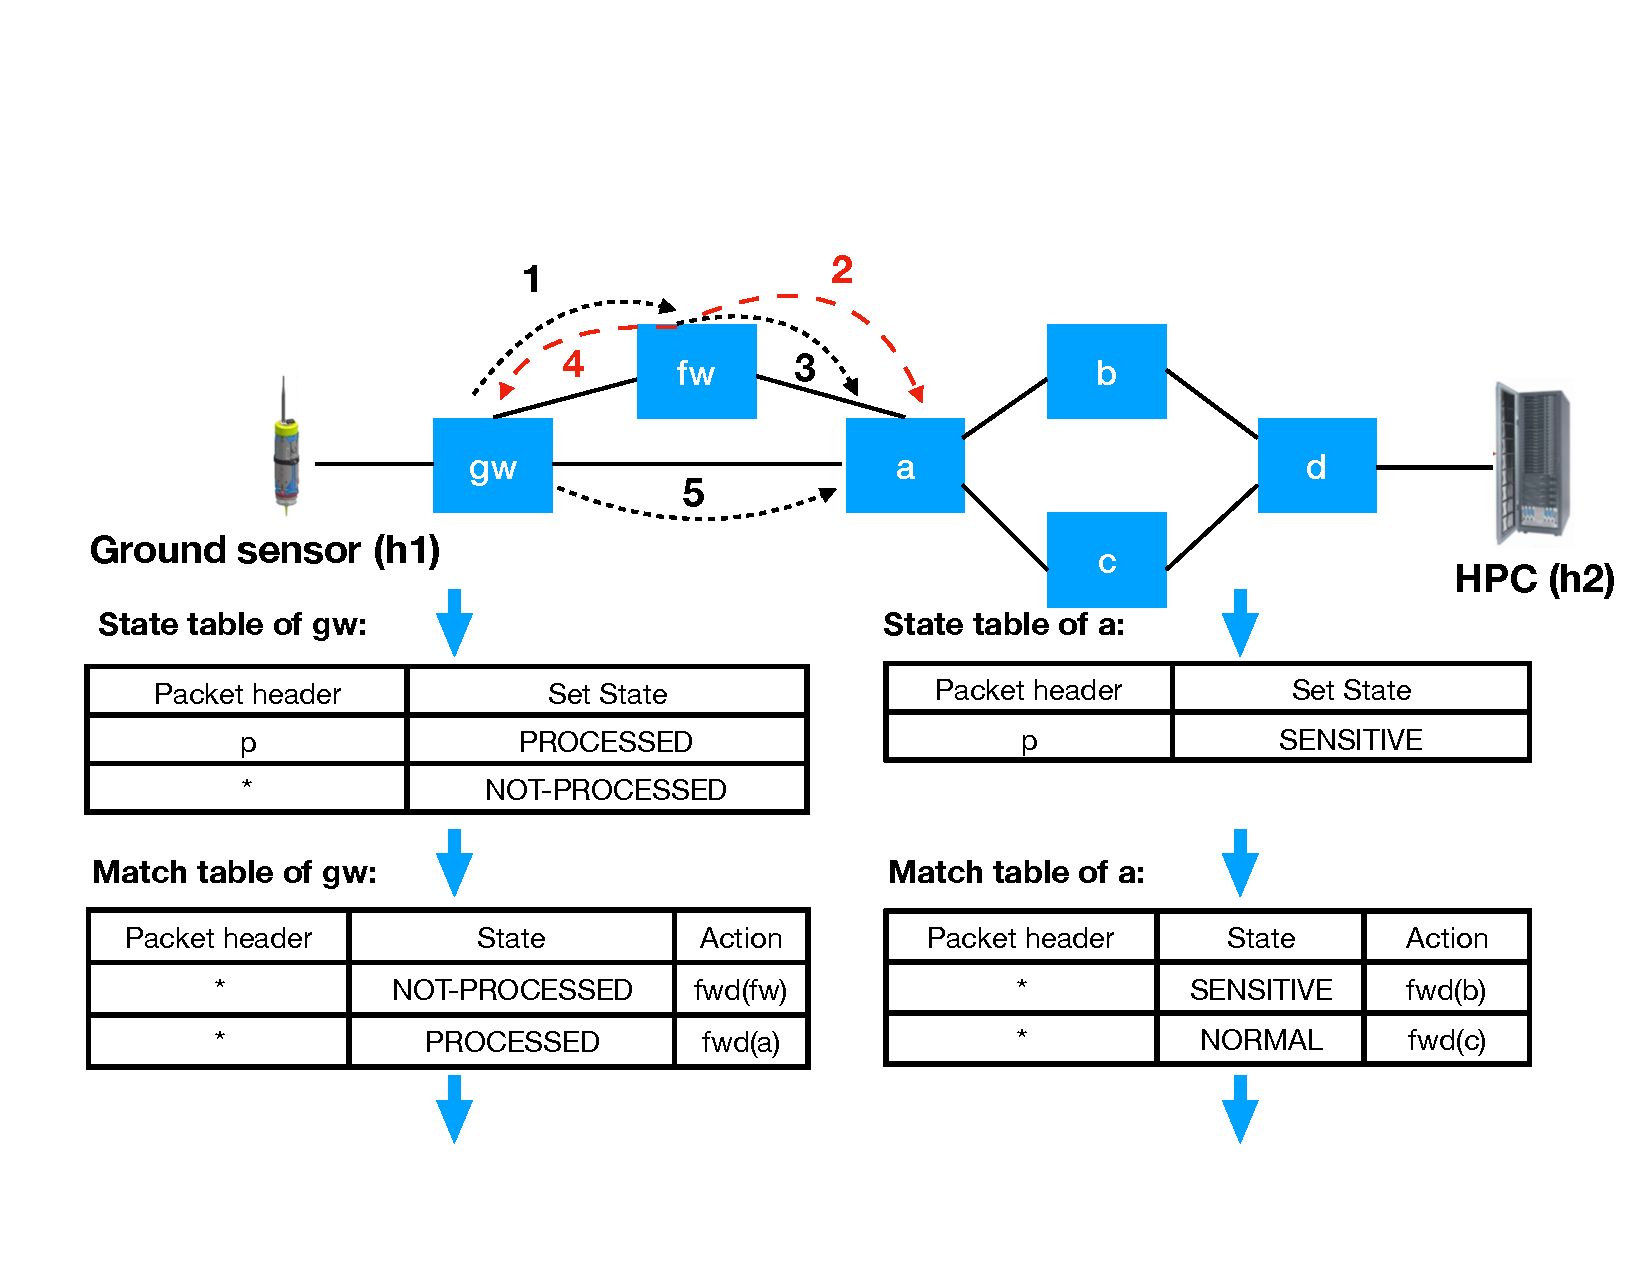
\includegraphics[width=\linewidth]{figures/ss-124.pdf}
%      \caption{\label{fig:dsdc-result} \small Configuration with \concept{}.}
%\end{subfigure}
%\vspace{-2mm}
%\caption{\footnotesize{The CDF of job latency local and remote jobs.}}
\caption{研究动机示例:一个SDC数据收集应用在一个具有防火墙的网络中。}
%\vspace{-2mm}
\label{fig:fw-example}
\end{figure}

\para{研究动机}: 
我们这里会通过一个例子来证明目前系统的限制,以及共享本地状态的好处。我们考虑图~\ref{fig:fw-example}(a)的一个战术网络,其中包括一个地面传感器($h_1$)一个防火墙中间盒($fw$)、一个计算服务器($h_2$)、一个网关交换机($gw$)、多个转发交换机($a$-$d$)。链路$gw\rightarrow fw$以及$fw \rightarrow a$的带宽为10 Kbps,而其他的链路均为100 Kbps。传感器$h_1$将数据收集后,首先转发到防火墙$fw$并基于数据包的五元组(即,srcAddr、dstAddr、srcPort、dstPort、protocol)判断该数据是否为敏感数据。同时SDC数据收集应用程序的目标是将传感器收集上的数据传到服务器上。而网络管理员对于数据传输有如下策略要求:对于任何从$h_1$传到$h_2$的数据,如果是敏感的,则数据应经过交换机$b$传输;否则经过交换机$c$传输。

%We give an example to demonstrate the limitation of existing systems, and the
%benefit of local state sharing. In particular, we consider a tactical network in
%Fig.~\ref{fig:fw-example}(a), which consists of a ground sensor ($h_1$), a
%middebox firewall ($fw$), a computing server ($h_2$), a gateway switch $gw$, and
%other forwarding switches ($a$-$d$). The bandwidth of links $gw\rightarrow fw$,
%and $fw \rightarrow a$ is
%10 Kbps, while the bandwidth of all other links is 100 Kbps. 
%The data collected by the sensor $h_1$
%should first be sent to the firewall $fw$, which identifies whether the data
%is sensitive or not based on the 5-tuple of
%the packet carrying the data (\ie, srcAddr, dstAddr, srcPort, dstPort and
%protocol). An SDC data collection application is running to send data collected
%from the sensor to the server. The network operator wants to enforce the following policy: For any
%data sent from $h_1$ to $h_2$, if it is sensitive, the
%data should be forwarded along a route passing switch $b$, otherwise passing switch $c$. 

为了保障这样的策略要求,目前已有的数据平面系统(例如,SNAP~\cite{arashloo2016snap})会给出如图~\ref{fig:fw-example}(b)的数据平面配置(这些数据平面系统均不支持在数据平面设备之间共享本地状态)。网关交换机$gw$将所有数据包转发至防火墙$fw$;防火墙$fw$根据其五元组判断数据流是否敏感,并根据判断结果添加相应的标签给所有的数据包,最后将数据包转发至交换机$a$;交换机$a$匹配数据包上的标签,并根据匹配结果转发至交换机$b$(沿着路径1)或交换机$c$(沿着路径2)。

%To enforce such a policy, state-of-the-art stateful datapath systems (\eg,
%SNAP~\cite{arashloo2016snap}), which do not support local state sharing between
%data plane devices, would compute the configuration as shown in
%Fig.~\ref{fig:fw-example}(b).  Specifically, the gateway switch $gw$ forwards
%all packets to the firewall $fw$. $fw$ identifies if it is sensitive or not, and
%appends a tag on each packet to indicate the identification result before
%sending to switch $a$. Switch $a$ then matches the tag of each arrival packet
%and forwards them to $b$ (path1) or $c$ (path2) based on the matching result.

虽然该配置是正确的,但其并没有充分利用SDC网络资源,从而影响数据收集应用程序的性能。一旦数据流是否敏感被防火墙$fw$判断后,该数据流的后续数据包则不需要再经过$fw$。这些后续数据包应沿着路径$gw, a, c, d$或$gw, a, b, d$从而得到更高的带宽。然而,该设计在没有防火墙$fw$和网关$gw$和交换机$a$之间共享本地状态下无法实现。

%Though this configuration is correct, it does not fully utilize the resources in
%SDC network, impairing the performance of the data collection application. Once
%the sensitivity of a data flow is identified by the firewall $fw$, no future
%packet of this flow needs to pass $fw$ again. Instead, they can be forwarded along path $gw, a, c, d $, or $gw, a, b, d$ with a higher transmission bandwidth. However, such a new
%forwarding configuration cannot be realized without local state sharing between
%the firewall $fw$, the gateway $gw$ and the switch $a$.

以上例子证明了在数据平面设备之间共享本地状态的好处。然后为了实现共享本地状态,手动地进行低级网络配置是花费时间并且非常容易出错的。因此,我们设计Dandelion,一个SDC编程系统来自动地从高级SDC程序转为支持共享本地状态的数据平面配置。

%The above example demonstrates the benefits of local state sharing between data
%plane devices in SDC. However, manually setting up the low-level configuration
%for local state sharing is too time-consuming and error-prone. As such, we
%design \concept, a novel SDC programming system to automatically translate
%high-level SDC programs into datapath configurations with local state
%sharing.

\section{Dandelion系统概述}

本节中,我们首先给出Dandelion的编程模型,再描述Dandelion的架构以及从高级SDC程序到支持共享本地状态的数据平面配置的转化流程。

%In this section, we first give the programming model of \concept{}, followed by
%its architecture, and the workflow to transform a high-level SDC program to
%datapath configurations with local state sharing.

\subsection{编程模型}

由于这里考虑的场景符合上一章中的部分可编程网络,即网络中包含具有特定、固定功能网络节点,如中间盒等,因此Dandelion采用上一章中提出的中间盒的原语,以及引入中间盒处理的抽象语法。

%Dandelion采用目前主流的高级SDN编程系统(XXX)的编程模型。其主要思想是逻辑上通过一个onPacket函数对每个数据包进行编程。除了对数据包头进行读或测试的基本原语操作外,Dandelion为了用户指定SDC网络中的中间盒设计了如下原语。第一个则是指定网络中的中间盒,\codeword{m = middlebox(name,
%property)}。其中property标识该中间盒是否有状态。第二个则是调用中间盒对数据包的处理,\codeword{m.handle(pkt)}。具体来说,我们考虑一个中间盒为一个数据包处理函数。它可以返回对收到的数据包进行处理的结果。对于一个无状态中间盒,如果两个数据包具有相同的五元组,则它们的返回结果也相同;对于一个有状态中间盒,由于数据包的处理会考虑中间盒的状态,即使两个数据包具有相同的五元组,它们的返回结果也不一定相同。

%\concept{} adopts an omnipotent programming model proposed in high-level SDN
%programming systems (\eg, Maple~\cite{maple}), which logically programs every single packet with an
%onPacket function. In addition to the primitives that read and test on packet
%headers, \concept{} designs the following primitives for users to model and
%specify middleboxes in SDC network. The first is to specify a middlebox in the network (\codeword{m = middlebox(name,
%property)}) where the property indicates the middlebox is stateless or not; The
%second is to
%invoke the packet handling of a middlebox (\codeword{m.handle(pkt)}).
%Specifically, we consider a middlebox as a packet handling function that can
%return the result for the incoming packet. For the stateless middlebox, if two
%packets have the same 5-tuple match fields, they always have the same
%results. For the stateful middlebox, this cannot be guaranteed as the packet
%processing depends on the state in the middlebox.

在Dandelion系统中,交换机和中间盒的交互是双向的。通过一个隧道,一个交换机可以将一个数据包送到一个中间盒并进行处理。待处理完数据包后,中间盒可以将数据包返回给交换机并与多个其他交换机共享该数据包的本地状态。而该过程对于用户是透明的,即用户不需要手动地对数据平面进行配置实现设备之间本地状态的共享。在下一节中我们会给出Dandelion是如何自动地将高级SDC程序转为支持共享本地状态的数据平面配置。

%In \concept{}, the interaction between switch and middlebox is bi-directional.
%A switch can send a packet to a
%middlebox for the processing through a tunnel. After the processing, the middlebox can send
%the packet back and share its local state of the packet %(5-tuple flow matches)
%with switches. In \concept{}, such interaction is transparent to the user so that
%the user does not need to manually configure the local state sharing between
%data plane devices. Instead, as we will show in the next section, \concept{}
%automatically translates high-level SDC programs into data plane configurations
%with local state sharing.

%除了中间盒原语之外,为了让用户指定数据包在网络传输的路径的约束,Dandelion也引入了路由代数(route algebra)原语(XXX)。图(XXX)给出了Dandelion编程模型的抽象语法。其中,对于路由代数表达式,我们采用了与(XXX)相同的结构。对于中间盒,编程人员可以指定其属性,即有状态或无状态。

%In addition to the middlebox primitives, \concept{} also adopts the route algebra
%primitive~\cite{gao2018t} for the user to specify path constraints for packets
%forwarding in SDC network. The abstract syntax of the \concept{} programming model
%is shown in Fig~\ref{fig:grammar1}. Specifically, for the route algebra expressions, we adopt the same in~\cite{gao2018t}. For the middlebox, programmers can specify its property, \ie, stateless or stateful. 


%\begin{figure}[ht]
%{%\small
%% \fontsize{10}{12}\selectfont 
%%\scriptsize
%%{\bf Abstract syntax:}
%%\vspace{-2mm}
%\[%\arraycolsep=1.4pt\def\arraystretch{2.2}
%\begin{array}{rclr}
%p &\bnfdef & \ONPKT\ \{I\},\ d_1,\ \ldots,\ d_n &(\textit{program})\\
%d &\bnfdef & x^r\ =\ r\  & (\textit{route algebra decl})\\
% & & \bnfalt x^m\ =\ middlebox(n,\ s) & (\textit{middlebox decl})\\
%I &\bnfdef & x\ =\ e & \\
% & & \bnfalt I;I &  (\textit{sequencing})\\
% & & \bnfalt x\ =\ x^m.handle(pkt) &  (\textit{middlebox operation})\\
% & & \bnfalt \ifelse{e^b}{I}{I} &  (\textit{conditional})\\ %\\ 
% & & \bnfalt \return{x^r} \bnfalt \return{r} &  (\textit{func return})\\ 
%% & & \bnfalt m[e_1, \dots, e_n] := e & (\textit{map update}) \\
%% & & \bnfalt s := s \cup \{e\} \bnfalt s := s - \{e\} & (\textit{set update}) \\
%e &\bnfdef & c \bnfalt x &  (\textit{consts, vars})\\
%%& & \bnfalt x^r  & (\textit{route algebra vars}) \\
%& & \bnfalt x^m & (\textit{middlebox vars}) \\
%& & \bnfalt pkt.a & (\textit{packet fields}) \\
%% & & \bnfalt e+e \bnfalt e*e \dots & (\textit{arith}) \\ 
%e^r & \bnfdef & e == e \bnfalt e \leq e \dots & (\textit{relational})\\
%e^b & \bnfdef & e^r \bnfalt e^r\ \&\ e^r \bnfalt e^r\ |\ e^r \dots & (\textit{boolean})\\
%(r &{\color{blue}{\in}}&\mathit{route\ algebra\ expressions}) & \\
%(c &{\color{blue}{\in}}& \mathit{strings}) & (\mathit{consts})\\
%(a &{\color{blue}{\in}}& \{ \mathit{macSrc}, \mathit{ipDst} \dots \}) & (\textit{packet fields})\\
%(n &{\color{blue}{\in}}& \mathit{strings})  &  (\textit{middlebox names})\\
%(s &{\color{blue}{\in}}& \{ \mathit{stateless},\mathit{stateful} \})  &  (\textit{properties})\\
%(x &{\color{blue}{\in}} & \{\tx_1,\tx_2,\dots,\ty_1,\dots\}) &  (\textit{variables})\\
%\end{array}\]}% small
%%\vspace{1mm}
%% \hrule
%%\vspace{-5mm}
%\caption{Dandelion abstract syntax.}
%\label{fig:grammar1}
%\end{figure}

\para{Dandelion程序示例}:对于章节~\ref{sec:motivation}的例子,网络管理员可以写如下Dandelion程序,来实现根据数据包是否携带敏感数据选择不同路径转发的策略。


%\para{Example \concept{} program:} Revisit the motivating example in Section~\ref{sec:motivation}, the network
%operator can specify the policy to forward packets of sensitive and non-sensitive data along different paths using the \concept{} program in Fig.~\ref{fig:code}.


\begin{figure}[h]
\begin{verbatim}
L1: mFW = middlebox("firewall", "stateless")
L2: PATH1 = h1 -> b -> h2 //b: waypoint
L3: PATH2 = h1 -> c -> h2 //c: waypoint
L4: //any: picking any path
L5: def onPacket(pkt):
L6:   if pkt.srcAddr == h1 & pkt.dsrAddr == h2:
L7:     if mFW.handle(pkt) == SENSITIVE:
L8:       return any(SPC.stable + PATH1)
L9:     else:
L10:      return any(SPC.stable + PATH2)
L11:  else: return DROP
\end{verbatim}
	\caption{对应研究动机例子的Dandelion程序。}
\label{fig:code}
\end{figure}

在上一章节中我们已经讨论了程序正确性的问题,并引入了SPC的概念,所以这里我们不对该程序进行过多说明。值得注意的是,由于Dandelion希望通过本地状态的共享,实现网络资源的充分利用。这会导致在系统的不同状态时,数据流会沿着不同路径传输。因此,这里需要对SPC进行拓展,引入稳定SPC(\codeword{SPC.stable})的概念。关于\codeword{SPC.stable}的定义会在随后章节中说明。

%
%其中第二(三)行指定了转发路径约束,即路径从$h_1$至$h_2$并需经过节点$b$ ($c$)。该约束并不代表一个具体转发路径,而是一个路径约束。在返回语句中通过\emph{any}的函数(定义在XXX的路由代数中),标明选出满足约束的任何一条路径。虽然编程模型非常直接简单,但由于引入中间盒对数据包的处理操作,而中间盒需要映射到网络的物理节点,系统需要保证程序的正确性。

%Specifically, line 2 (3) specifies a path constraint that starts from $h_1$ to $h_2$ and must pass through $b$ ($c$) (Note that it does not represent a concrete path but a path constraint). And the return statements use \emph{any} function (defined in route algebra~\cite{gao2018t}) that picks any path satisfying the constraint. Although the programming model is quite simple, as involving middleboxes which physically map to nodes in the network, the system needs to guarantee the correctness for the program.

%\para{正确性}:我们采用如下对于正确性的定义:对于任何数据包$pkt$,其相应的在网络中的真实转发路径必选要符合程序中返回的对数据包$pkt$的路径。例如,如果程序员使用\emph{opt}函数来选择一个满足约束的最短跳数路径,即\codeword{opt(PATH1)}),则真实转发路径应为网络中的$gw, a, b, d$。然而,由于(第一个)数据包必须要经过防火墙,其真实转发路径必须包含防火墙$fw$,从而不符合程序中返回的路径。

%\para{Correctness}: We denote the correctness as the following: For any packet $pkt$, the real forwarding path for $pkt$ in the network must comply with the returned path for $pkt$ in the program. For example, if the programmer uses \emph{opt} function to pick the shortest hop count path with the constraint (\ie, \codeword{opt(PATH1)}), then the returned path is $gw, a, b, d$. However, as the (first) packet must access the firewall, the real path must include $fw$ which does not comply with the returned path in the program.

%为了保证正确性,一个简单的做法是让程序员显示地在路径约束上包含需要的中间盒节点。在上述场景中,其应为\codeword{PATH1 = h1 -> fw -> b -> h2}。然而,让程序员保证路径约束和网络中真实转发的一致性的做法,会给程序员带来额外的负担。

%One simple solution to guarantee the correctness is to let the programmer explicitly include the necessary middlebox nodes in the path constraint. In this case, it should be \codeword{PATH1 = h1 -> fw -> b -> h2}. However, this can add extra burden to programmers that they should make sure the path constraints comply with the traces of packets in the network.

%\para{系统路径约束}:为了解决上述问题,我们引入系统路径约束(System Path Constraint,SPC)的概念。在程序中,SPC表示为一个存有路径约束的全局变量。程序中的任何一个位置计算路径时需要满足SPC中的路径约束。其直观理解是,当一个数据包经过程序时,某些程序语句会给数据包添加路径约束。例如,图(XXX)中的第六行添加了一个从$h_1$到$h_2$的路径约束;第七行添加了一个必须要经过防火墙的路径约束。因此,在第七行后,SPC全局变量包含如下约束:从$h_1$到$h_2$以及经过防火墙$fw$。如果第八行中使用\emph{opt}函数计算路径,则应为\codeword{return opt(SPC + PATH1)},其中``+''表示连接SPC的路径约束和PATH1的路径约束,而其结果为$gw, fw, a, b, d$。(关于\codeword{SPC.stable}的定义会在随后章节中说明。)

%\para{System Path Constraint}: To resolve the issue, we introduce the System Path Constraint (SPC) which is a global variable storing path constraints that must be complied with when computing a path at any location in the program. The intuition is that when a packet going through the program, some statements can add path constraints for the packet. For example, in Fig.~\ref{fig:code}, line 6 adds a constraint that the path should start from $h_1$ to $h_2$; Line 7 adds a constraint that the path must include the firewall. Then, after line 7, the SPC variable includes constraints that the path starts from $h_1$ to $h_2$ and includes $fw$. If the line 8 uses the \emph{opt} function, then it should be \codeword{return opt(SPC + PATH1)} where the ``+'' means connecting the waypoints constraints in SPC and PATH1, and its result is $gw, fw, a, b, d$. (Note that the definition of \codeword{SPC.stable} will be given in the next section.)


%
%\begin{figure}[h]
%\begin{footnotesize}
%\begin{verbatim}
%L1: mFW = middlebox("firewall")
%L2: PATH1 = h1 -> mFW -> b -> h2 //b: waypoint
%L3: PATH2 = h1 -> mFW -> c -> h2 //c: waypoint
%L4: opt := picking shortest hop count path
%L5: def onPacket(pkt):
%L6:     if pkt.srcAddr == h1 & pkt.dsrAddr == h2:
%L7:         if mFW.handle(pkt) == SENSITIVE:
%L8:             return opt(PATH1) 
%L9:         else:
%L10:           return opt(PATH2)
%L11:    else: return DROP
%\end{verbatim}
%\end{footnotesize}
%	\caption{\small The \concept{} program for the policy in the motivating example.}
%\label{fig:code}
%\end{figure}
%
%\begin{figure}[h]
%\begin{footnotesize}
%\begin{verbatim}
%L1: mFW = middlebox("firewall")
%L2: PATH1 = h1 -> b -> h2 //b: waypoint
%L3: PATH2 = h1 -> c -> h2 //c: waypoint
%L4: opt := picking shortest hop count path
%L5: def onPacket(pkt):
%L6:     if pkt.srcAddr == h1 & pkt.dsrAddr == h2:
%L7:         if mFW.handle(pkt) == SENSITIVE:
%L8:             return opt(SPC.stable + PATH1) 
%L9:         else:
%L10:           return opt(SPC.stable + PATH2)
%L11:    else: return DROP
%\end{verbatim}
%\end{footnotesize}
%	\caption{\small The \concept{} program for the policy in the motivating example.}
%\label{fig:code}
%\end{figure}


%
%Also, as only stateless middleboxes can leverage stateful switches as the cache of results of its packet processing, the system needs to identify whether a middlebox is stateless or not. For simplicity, we make the programmer give the hint. In the program, when initializing a middlebox variable, the program should specify whether it is stateless or not. The following gives an example that how to give a hint at the middlebox variable initializing statement.
%
%\begin{small}
%\begin{verbatim}
%mFW = middlebox("firewall", "stateless")
%...
%if mFW.handle(pkt) = GOOD:
%\end{verbatim}
%\end{small}
%

\subsection{系统架构以及工作流程}

图~\ref{fig:system-workflow}给出了如何从高级Dandelion程序到支持共享本地状态的低层次数据平面配置的架构以及流程。给定一个高级Dandelion SDC程序,Dandelion首先计算出对应的决策图。该决策图包含了程序对数据包的决策过程以及相应的有状态操作。其次,Dandelion根据系统优化目标(例如,吞吐量最大化),算出网络中的转发路径。需要注意的是,只有当程序中返回的路径不是具体路径时(例如,使用$any$函数计算路径),系统才需要计算路径。而当返回的路径为具体路径时(例如,使用$opt$函数计算路径),系统不需计算路径。最后,生成相应的设备级别数据平面配置,并包含共享本地状态的配置以实现设备之间可以共享本地状态。Dandelion利用有状态交换机来实现共享本地状态。有状态交换机的基本模型为两张匹配操作表(match-action):第一张为状态表,即匹配数据包头并返回状态($match \rightarrow state$);第二张为匹配表,即匹配数据包头以及状态并返回操作($match+state \rightarrow action$)。当数据包到达一个有状态交换机时,首先进入状态表并根据数据包头来获取相应的状态,再进入匹配表来得到操作。

%\subsection{Architecture and Workflow}
%Fig.~\ref{fig:system-workflow} presents the architecture and workflow on how
%\concept{} translates high-level \concept{} SDC programs to low-level
%configurations of data plane devices with local state sharing. Given a
%high-level \concept{} SDC program, \concept{} first computes a decision graph that captures the forwarding decisions process of
%packets and stateful operations on packets. Second, \concept{} computes optimal
%paths for packet forwarding in the network with a system defined objective (\eg,
%maximizing total throughput). \textbf{Note} that the system computes paths when the returned paths are not concrete (\eg, using $any$ function), and in the remaining part of the paper, we assume these paths are not concrete to introduce the path computation part. Third, the device-level data plane configurations are generated, which
%include local state sharing configurations, so that devices can exchange local
%state to forward the packets along the computed optimal paths. \concept{} leverages the stateful switch for local state sharing which includes two match-action tables: one is
%a state table (\ie, $match \rightarrow state$) and the other is a match table
%(\ie, $match+state \rightarrow action$). Given a switch, a
%packet first enters the state table to get its corresponding state (by matching
%its packet fields) and then enters the match table to get the action.

\begin{figure}[!htbp]
%\vspace{-2mm}
\centering

      \centering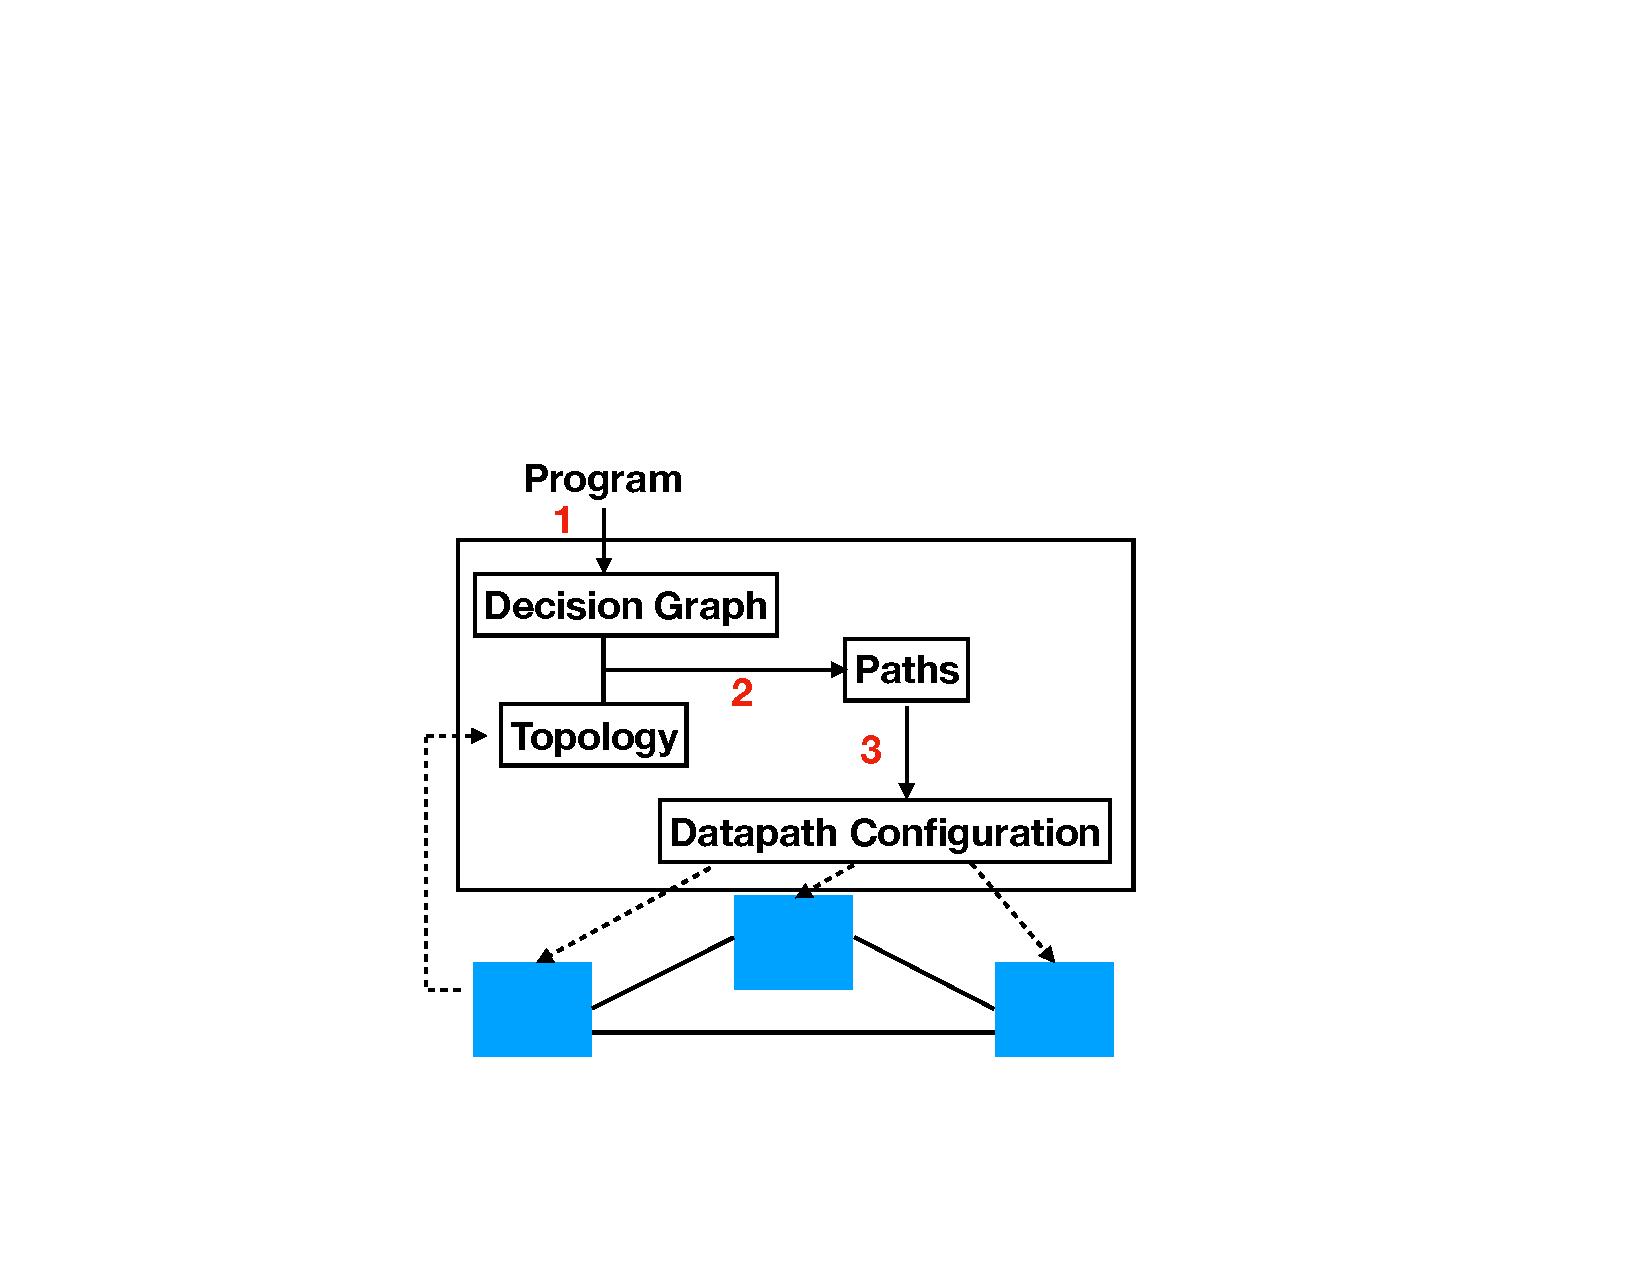
\includegraphics[width=\linewidth]{figures/ss-125.pdf}
%\vspace{-2mm}
%\caption{\footnotesize{The CDF of job latency local and remote jobs.}}
\caption{Dandelion架构以及工作流程。}
%\vspace{-2mm}
\label{fig:system-workflow}
\end{figure}

\begin{figure}[!htbp]
%\vspace{-2mm}
\centering
      \centering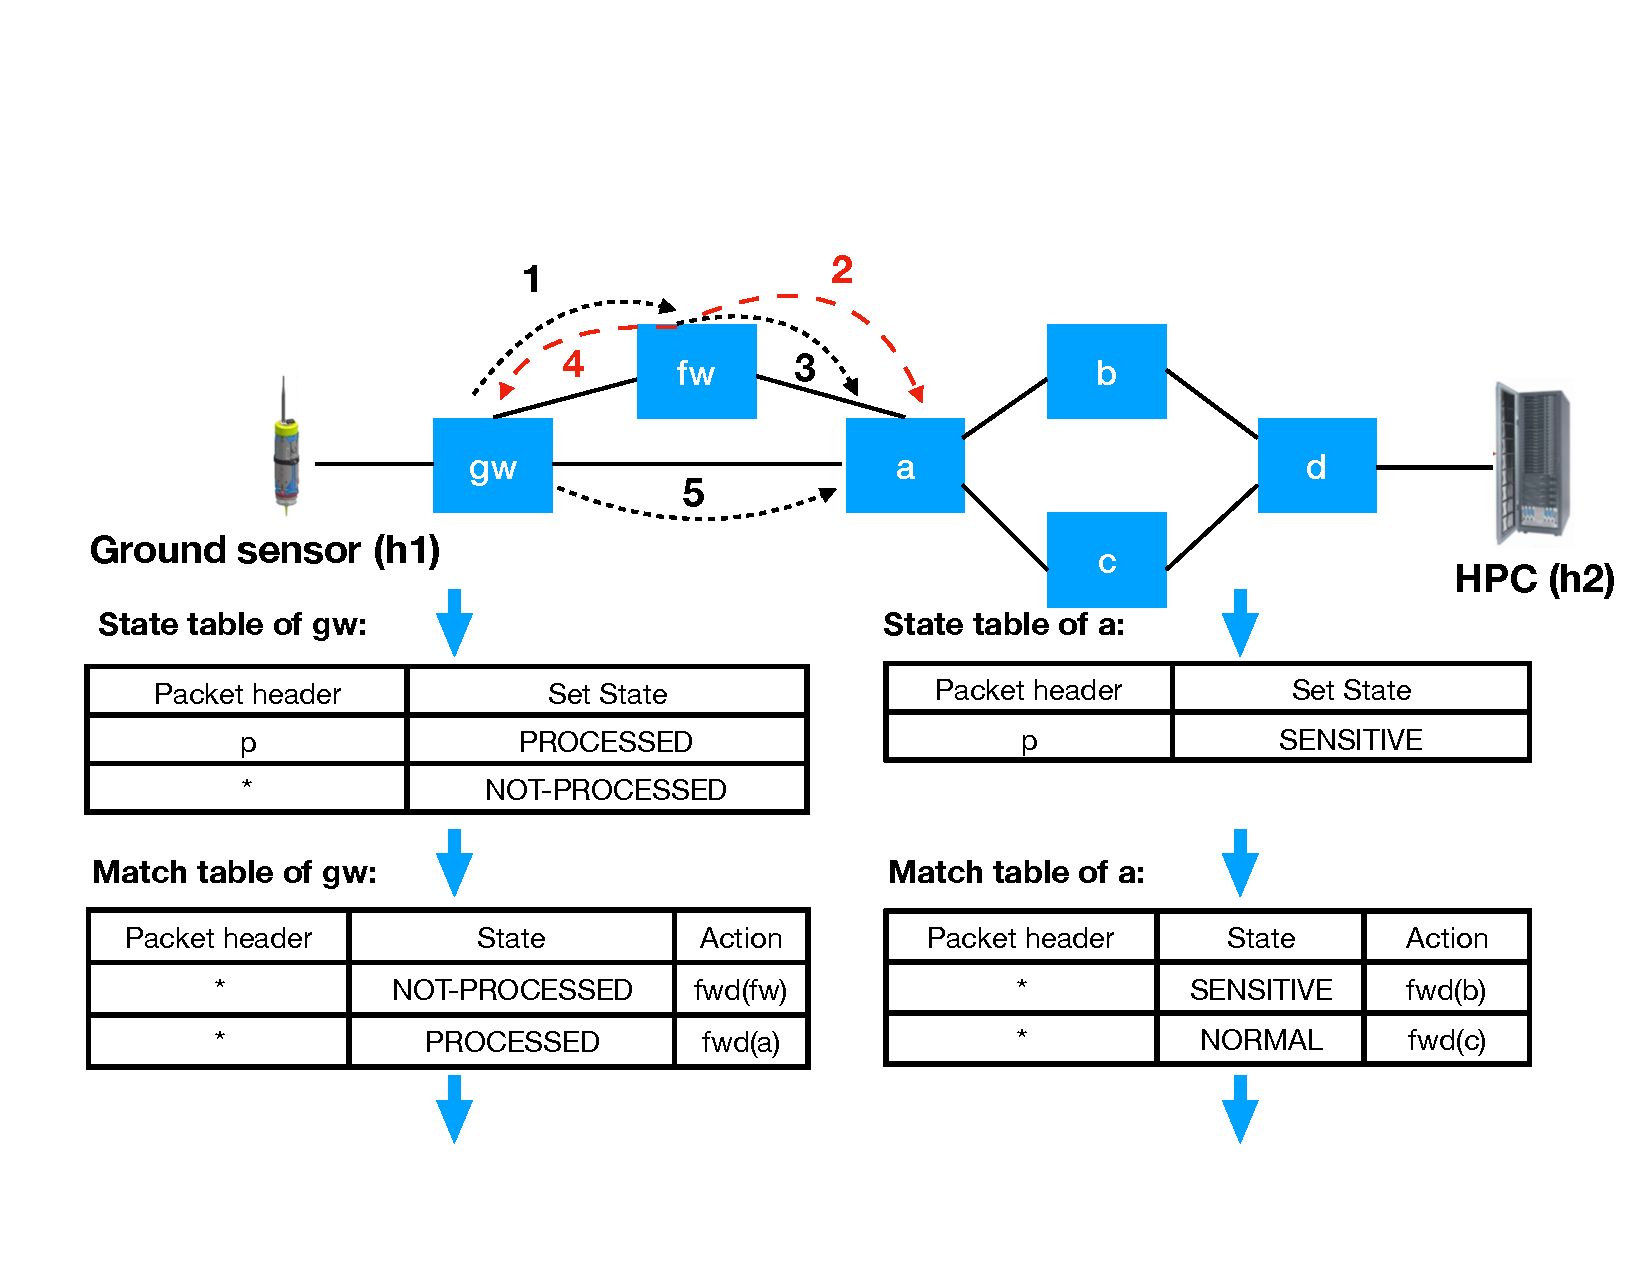
\includegraphics[width=0.8\linewidth]{figures/ss-124.pdf}
   %\vspace{-2mm}
%\caption{\footnotesize{The CDF of job latency local and remote jobs.}}
	\caption{从图~\ref{fig:code}中程序转换后的配置。}
%\vspace{-2mm}
\label{fig:dsdc-result}
\end{figure}

\para{支持共享本地状态的配置示例}:图~\ref{fig:dsdc-result}给出了从图~\ref{fig:code}的SDC程序生成的支持共享本地状态的数据平面配置。具体来说,通过允许共享本地状态,防火墙$fw$可以将对数据流标识的状态传给网关交换机$gw$。例如,它可以发送如下状态信息:$srcAddr=h1,dstAddr=h2,srcPort=12345,dstPort=22,protocol=tcp \rightarrow$
\emph{PROCESSED}给$gw$。网关$gw$可以将其设置在状态表中。

%\para{Example configuration with local state sharing}:  
%Fig.~\ref{fig:dsdc-result} gives the data plane configuration with local state
%sharing translated from the SDC program in Fig.~\ref{fig:code}. Specifically,
%by allowing the local state sharing, the
%firewall $fw$ can share its local identification state for a flow with the
%gateway switch $gw$.
%For example, it can send the state: 
%$srcAddr=h1,dstAddr=h2,srcPort=12345,dstPort=22,protocol=tcp \rightarrow$
%\emph{PROCESSED} to $gw$, which can insert it into its state table.

根据此配置,第一个到达网关$gw$的数据包$pkt$会被传送到$fw$来得到状态\emph{NOT-PROCESSED}(第一步)。假设$fw$识别$pkt$为\emph{SENSITIVE}。则$fw$会首先发送该状态信息$pkt \rightarrow SENSITIVE$给交换机$a$(第二步)。其次,$fw$会转发$pkt$到$a$(第三步)。在交换机$a$,由于$pkt$的状态为\emph{SENSITIVE},$pkt$会转发给$b$。最后,$fw$共享本地状态$pkt \rightarrow PROCESSED$到网关$gw$(第四步)。而随后的与$pkt$具有相同匹配字段的数据包到达$gw$后会直接转发到交换机$a$(第五步)。

%With this configuration, the first packet $p$ arrives at the
%gateway $gw$ is forwarded to $fw$ by getting a state
%\emph{NOT-PROCESSED} at $gw$ (Step 1). Assume $fw$ identifies $p$ as \emph{SENSITIVE}.
%It first sends this local state $p \rightarrow SENSITIVE$ to $a$ (Step 2). Next,  $fw$
%forwards $p$ to $a$ (Step 3), where $p$ is forwarded to $b$ because its state is \emph{SENSITIVE}. 
%Then $fw$ sends the local state $p \rightarrow PROCESSED$ to $gw$ (Step 4). As such, all future packets with the
%same match fields as $p$ entering $gw$ will be forwarded directly to $a$ (Step 5).


\section{Dandelion设计细节}

在本节中,我们给出Dandelion的细节部分:决策图,路径计算,以及数据平面配置的生成。

%In this section, we present the details of \concept{}. We
%first give the details of decision graph, followed by the path
%computation and the data path generation. 

\subsection{决策图}

决策图(Decision Graph,DG)用来捕获数据包的转发决策过程以及对数据包的有状态操作。我们定义DG为一个单根有向无环图。该图有三种节点:数据包(packet-test)测试节点,中间盒处理(middlebox-operation)节点,以及操作(action)节点(分别映射三个基本原语:数据包测试,中间盒处理,以及路由代数)。数据包测试本质上与数据包的读取一样,为了便于理解,我们采用数据包测试。前两个节点为DG的内部节点;后一个为叶子节点。如果一个节点为数据包测试节点,则其出边标识了数据包的域的范围;如果一个节点为中间盒处理节点,则其出边标识了对数据包的处理结果。例如,图~\ref{fig:dg-example}给出了研究动机程序的相应的DG。本工作中,我们不关注如何生成DG。DG的计算可以参考已有的相关工作~\cite{arashloo2016snap}~\cite{smolka2015fast}。

%The Decision Graph (DG) is used to capture the forwarding decisions process of
%packets and stateful operations on packets. 
%We define a DG as a directed acyclic graph (with a single root) that has three types of nodes: packet-test nodes, middlebox-operation nodes, and action nodes (mapping to three basic primitives, packet-test, middlebox, and route algebra). The first two nodes are the internal nodes of DG while the last one is the leaf node. An out-edge of a node can specify a range of packets (if the node is a packet-test node) or a result from a middlebox (if the node is a middlebox-operation node). For example, the DG of the motivating program is shown in Fig.~\ref{fig:dg-example}. Note that we do not focus on the computation of DG from a program which can be achieved by existing (compiler) work~\cite{arashloo2016snap}~\cite{smolka2015fast}.

\begin{figure}[!htbp]
%\vspace{-2mm}
\centering
      \centering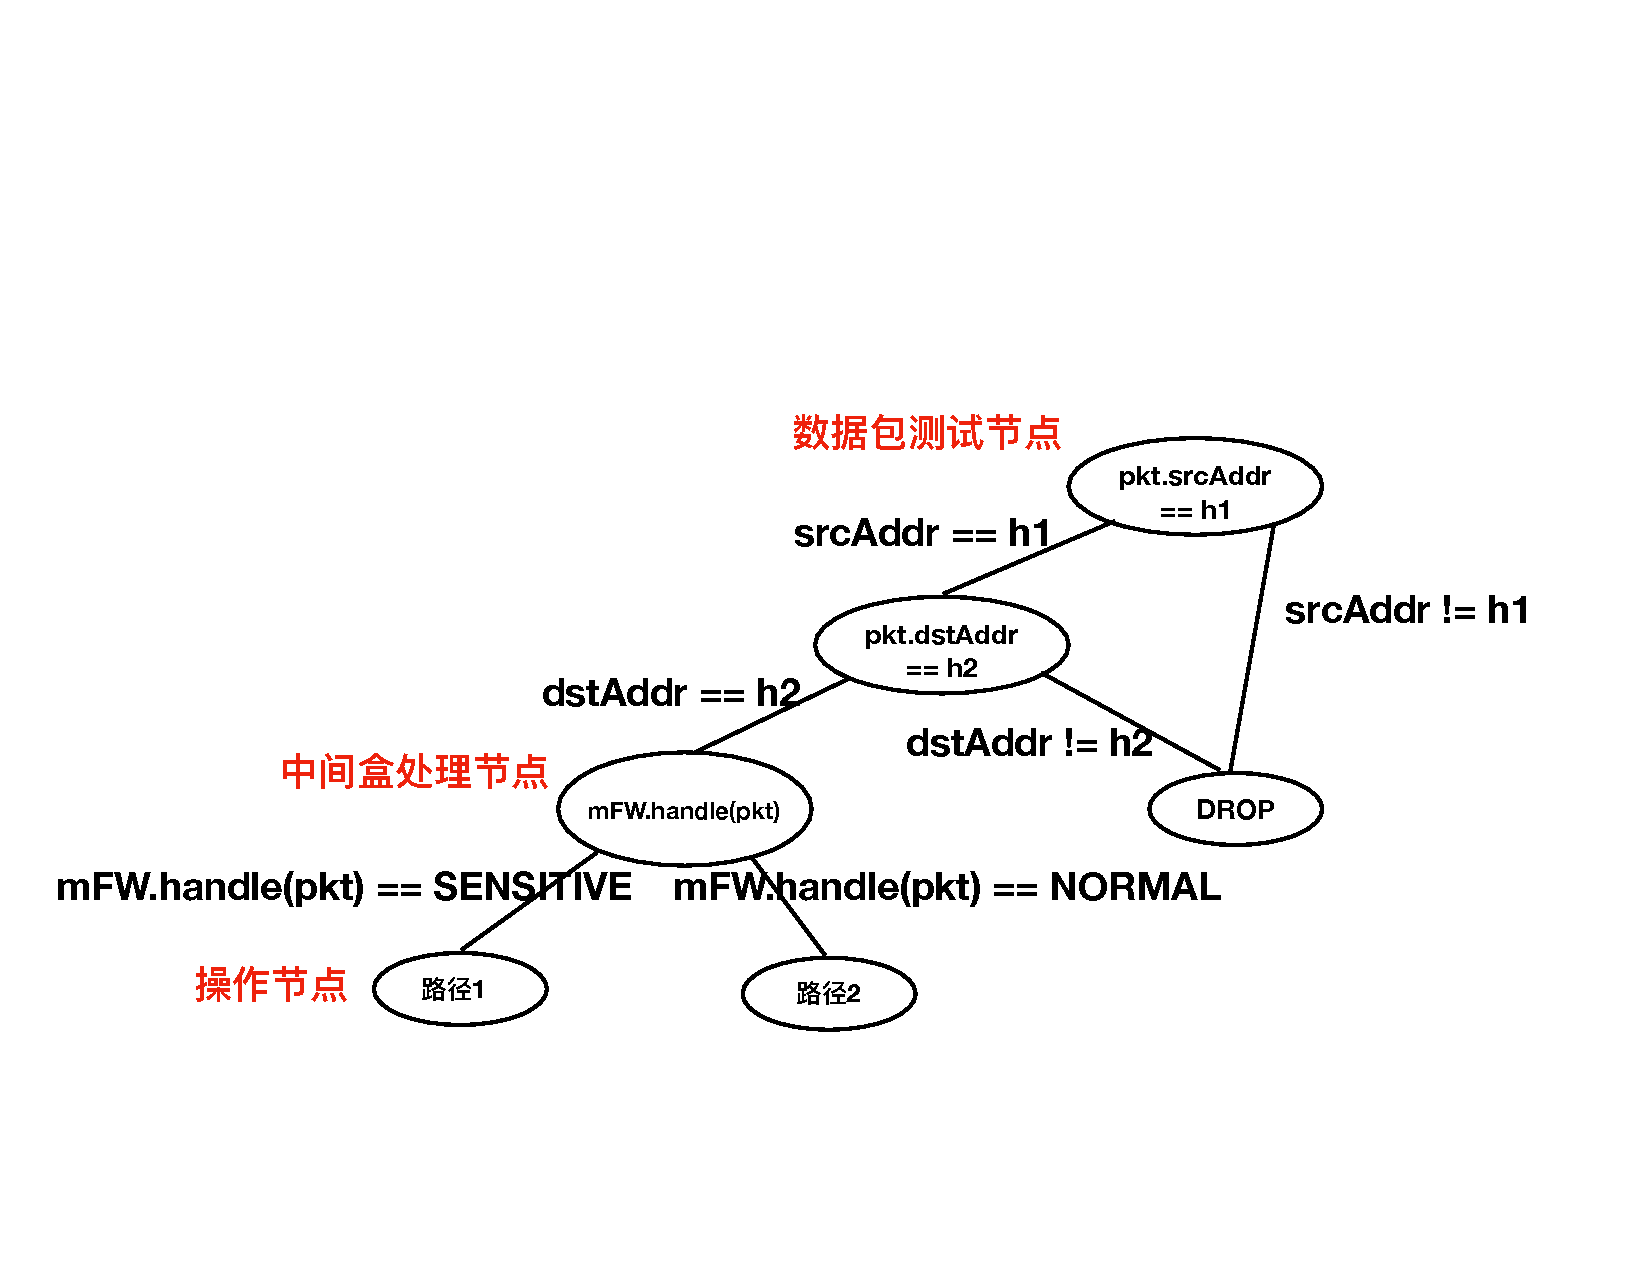
\includegraphics[width=\linewidth]{figures/ss-126.pdf}
\caption{DG示例。}
%\vspace{-2mm}
\label{fig:dg-example}
\end{figure}

给定一个DG,对于从根节点到一个操作节点(即路径约束,path constraint)$pc$的节点和边的序列,我们称之为$pc$的踪迹(trace),即$T(pc)$。给定一个踪迹$T(pc)$,我们称$T(pc)$中的中间盒处理节点为$M(pc)$。因为中间盒处理节点代表实际网络中中间盒对数据包的处理操作,为了不形成环,在$M(pc)$中每个中间盒节点只可以出现一次。并通过从$M(pc)$抽取代表有状态中间盒的中间盒操作节点,我们可以得到一个$M(pc)$的子序列(称为$M^s(pc)$)。该子序列$M^s(pc)$中的每个节点代表有状态中间盒的操作。给定一个$T(pc)$,对于其操作节点的SPC可以由$T(pc)$(包含了数据包到达该操作节点的踪迹)简单地计算出来。

%Given a DG, we denote the sequence of nodes and edges from the root to an action node (\ie, path constraint $pc$) as the trace of $pc$ ($T(pc)$). Then, given a trace $T(pc)$, we denote the middlebox-operation nodes of $T(pc)$ as $M(pc)$ (\ie, a sequence of nodes). As middlebox-operation nodes represent the packet handling of middleboxes, to not form loops, every middlebox-operation node can only appear once in $M(pc)$. Also, by extracting middlebox-operation nodes that represent stateful middleboxes from $M(pc)$, we have a subsequence of $M(pc)$ that every node is for stateful middlebox operations (denoted by $M^s(pc)$). Given a $T(pc)$, the SPC for its action node can be easily computed as the $T(pc)$ gives the trace of the packet enters the action node.

\subsection{路径计算}

由于DG的叶子节点代表路径约束,路径计算的目标则是根据系统性能目标对这些叶子节点计算出具体路径。(如果叶子节点为具体路径,则跳过路径计算过程。)

%As the leaf nodes in DG are path constraints, path computation targets to compute the concrete paths for these leaf nodes with a system performance objective. (And if leaves are concrete paths, the path computation just skips them.)

\para{数据包转发模型}:在路径计算之前,我们首先给出在网络中的基于DG的数据包转发模型。如图~\ref{fig:pfm-example}所示,给定在研究动机例子中的一条路径($gw, a, b$),逻辑上该路径上的每一个交换机都保存该示例程序的DG。其中$P$表示数据包测试节点;$M$表示中间盒处理节点;$A$表示操作节点。红色的$A$节点表示该路径的相应的约束。如图红色线所示,到达网关$gw$的数据流的第一个数据包开始遍历DG。当数据包遇到一个中间盒节点时,通过一个隧道,它会被送到相应的中间盒。待处理完成后,中间盒会将数据包返回并共享其本地状态(即添加或修改状态表的流规则)给路径沿途上的交换机的相应的中间盒处理节点(每个节点可以被看作为一对状态和匹配表)。如果中间盒为有状态中间盒,则不设置状态,而让数据包携带状态。待遍历完DG后(即沿着红色线到达叶子节点),数据包得到一条路径并根据路径进行转发。由于本地状态已经共享给了其他交换机的相应的中间盒处理节点(或对于有状态中间盒,则携带在数据包上),数据包在随后的交换机中无需再送给中间盒进行处理。

如果数据包没有经过任何无状态中间盒(相比第一个数据包需要经过这些无状态中间盒),我们称该数据包的转发为稳定的(stable)。根据稳定转发的定义,我们拓展原始的SPC变量为\codeword{SPC.stable}。该拓展后的变量表示只保留稳定转发路径的约束(即去除无状态中间盒)。因此,为了支持共享状态,由于\codeword{SPC}包括了所有数据包(含第一个数据包要经过的所有中间盒)的全部的约束,程序中应该使用\codeword{SPC.stable}而非\codeword{SPC}。

%\para{Packet forwarding model}: Before path computation, we first give a packet forwarding model with DG in the network as the following. As shown in Fig.~\ref{fig:pfm-example}, given a path ($gw, a, b$) in the motivating example, logically we consider every switch in the path has the DG of the example program where $P$ indicates a packet-test node, $M$ indicates a middlebox-operation node, and $A$ indicates an action node. The $A$ node with red color represents the corresponding constraints for the path. The first packet of the flow (arriving at $gw$) starts to traverse the DG as the red line in the figure. When the packet meets a middlebox-operation node, it will be sent to the corresponding middlebox through the tunnel. After the processing, the middlebox will send the packet back and share its local state (\ie, by installing/modifying rules in the state table) for the flow with the corresponding middlebox-operation nodes (each node can be viewed as a pair of state table and match table) at switches along the path. (If the middlebox is stateful, then it does not set any state but makes the packet carry the state.) After the traversal of the DG (\ie, arriving at the leaf node along the red line), the packet will get the path and should be forwarded along the path. As local states have been shared with corresponding middlebox-operation nodes (or carried by the packet for stateful middleboxes) at other switches, the packet does not need to be sent to the middlebox again at the next switch. We denote a forwarding of a packet as stable forwarding if the packet does not access any stateless middlebox (compared with the first packet that should access them). Based on the stable forwarding, we can extend original SPC variable to \codeword{SPC.stable} which means the system path constraints only for stable forwarding paths (\ie, remove the stateless middleboxes). Then, to allow the state sharing, \codeword{SPC.stable} should be used as \codeword{SPC} includes the whole constraints for all packets including the first packet that must pass through all the middleboxes.

\begin{figure}[!htbp]
%\vspace{-2mm}
\centering
      \centering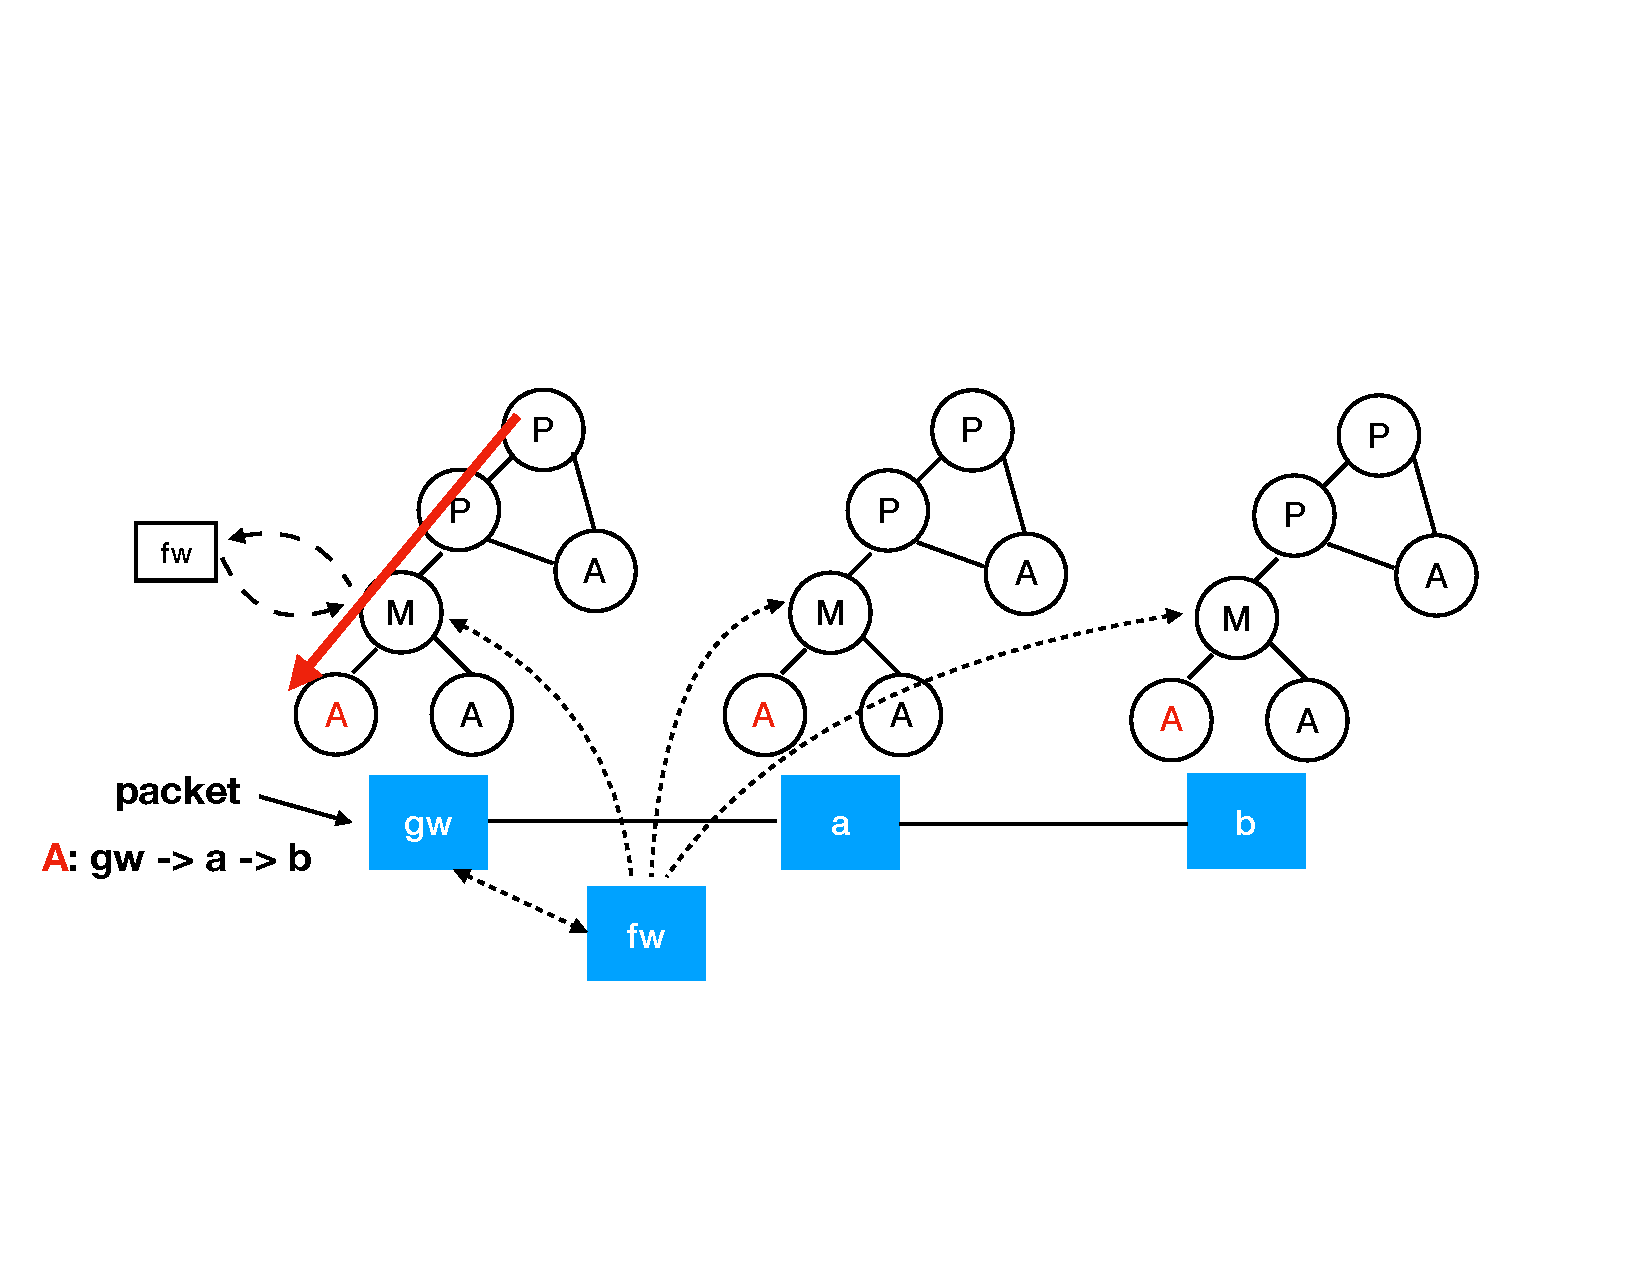
\includegraphics[width=\linewidth]{figures/ss-127.pdf}
\caption{基于DG的数据包转发模型。}
%\vspace{-2mm}
\label{fig:pfm-example}
\end{figure}

\para{系统目标}:基于转发模型,由于数据传输最初的一些数据包对整个数据流传输的影响较小,一个简单的路径计算(即只考虑稳定转发)如下所述。我们考虑系统目标为吞吐量的最大化,即,maximize $\sum_ib_i$。其中$i$表示路径约束$pc_i$的标号,$b_i$为其吞吐量。表~\ref{table:variables}给出了变量的定义。表~\ref{table:constraints}给出了约束(其中$Path(x, y, E)$表示$E$中存在一条从$x$到$y$的简单路径)。本工作中,对于路径约束,我们关注基准点(waypoint)约束(因为这种约束会给路径计算带来复杂性)。我们考虑基准点约束为一组节点对。节点对的形式为$(x, y)$,表示数据包要先经过$x$再到$y$。($x$和$y$可以为源或目的节点。)

%\para{System objective}: Based on the model, as the forwarding of the first few packets has little influence on the performance of the flow, a simple path computation (that only considers the stable forwarding) would be the following. We consider the objective of the network is to maximize the total throughput, \ie, maximize $\sum_ib_i$ where $i$ is the index of the path constraint $pc_i$ and $b_i$ is its throughput. The definition of variables can be found at Table~\ref{table:variables}. And the constraints can be found at Table~\ref{table:constraints} (where $Path(x, y, E)$ means there exists a simple path starting from $x$ to $y$ in $E$). In this paper we focus on the waypoints constraints for the path constraints (as they may complicate the path computation) and we consider the waypoints constraint as a set of node pairs where a pair has the form $(x, y)$ which indicates packets must pass through $x$ before $y$. (Note that $x$ and $y$ can be source/destination nodes.)

\begin{table}[]
\begin{tabular}{l|l}
变量     & 含义                                                             \\ \hline
$u_i$, $v_i$ & 路径约束$pc_i$的源和目的节点                            \\ 
$E$          & 网络中所有的边(其中一个边表示为$e$: $(e.src, e.dst)$)                       \\
$m_e$        & 边$e$的最大带宽                                            \\
$W_i$        &  $pc_i$的一组节点对\\
$z^i_e$      &  $pc_i$选出的边$e$\\
$b_i$          & 使用$pc_i$的流的带宽                            
\end{tabular}
\caption{变量及其含义。}
\label{table:variables}
\end{table}

%\begin{table}[]
%\scriptsize
%\begin{tabular}{l|l}
%Variable     & Description                                                             \\ \hline
%$u_i$, $v_i$ & The source and destination nodes of path constraint $pc_i$                            \\ 
%$E$          & All edges (an edge $e$: $(e.src, e.dst)$) in the network                       \\
%$m_e$        & The maximum bandwidth of $e$                                            \\
%$W_i$        & A set of node pairs of $pc_i$ \\
%$z^i_e$      & The edge $e$ is selected by $pc_i$ \\
%$b_i$          & The bandwidth of flows using the path for $pc_i$                                   
%\end{tabular}
%\caption{\small Notation.}
%\label{table:variables}
%\end{table}

\begin{table}[]
\begin{tabular}{l|l}
约束                                        & 含义                               \\ \hline
$\forall i, \forall (x, y) \in W_i, Path(x, y, E)$                    & 路径约束                  \\
$\forall i, Path(u_i, v_i, E)$      & 路径存在于$E$     \\
$\forall e \in E, \sum_ib_i*z^i_e \le m_e$   & 边的带宽约束
\end{tabular}
\caption{约束及其含义。}
\label{table:constraints}
\end{table}

%\begin{table}[]
%\scriptsize
%\begin{tabular}{l|l}
%Constraint                                        & Description                               \\ \hline
%$\forall i, \forall (x, y) \in W_i, Path(x, y, E)$                    & Path constraints                  \\
%$\forall i, Path(u_i, v_i, E)$      & Path exists in $E$     \\
%$\forall e \in E, \sum_ib_i*z^i_e \le m_e$   & Bandwidth constraints for edges
%\end{tabular}
%\caption{\small Constraints.}
%\label{table:constraints}
%\end{table}

由于通过使用\codeword{SPC.stable},系统路径约束已经添加到了路径约束中,正确性已经可以保证。即数据包先得到有状态中间盒的处理结果,然后选择正确路径。

%As the system path constraints have been added into the path constraints (by using the \codeword{SPC.stable}), the correctness can be guaranteed. And it enforces a packet must get results of stateful middleboxes and then select the correct path.

\begin{figure}[!htbp]
%\vspace{-2mm}
\centering
      \centering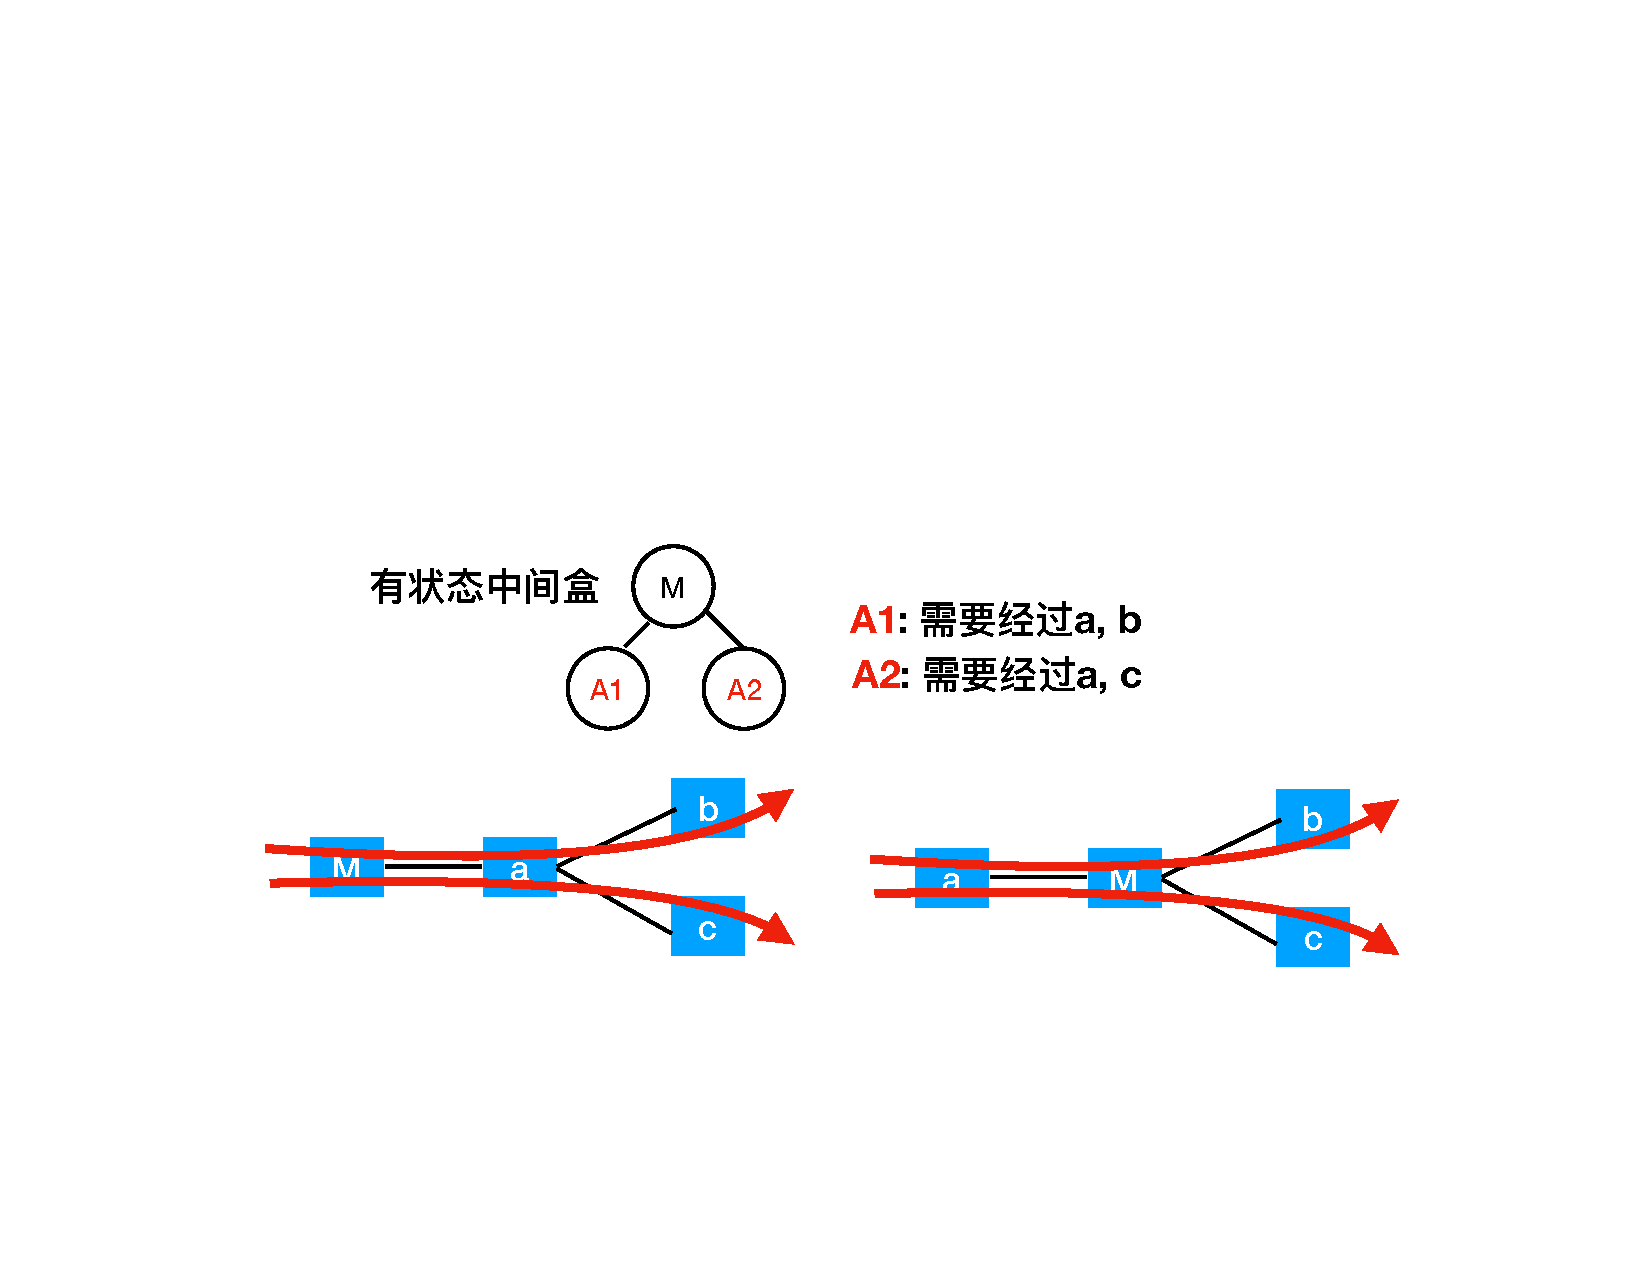
\includegraphics[width=\linewidth]{figures/ss-128.pdf}
\caption{两种转发路径均满足要求。}
%\vspace{-2mm}
\label{fig:c-example}
\end{figure}

然而,当前的路径约束可能会导致``过度约束"的问题。例如图~\ref{fig:c-example},一个有状态中间盒处理节点$M$有两个路径约束$A_1$和$A_2$作为其DG中的子节点。并且$A_1$要求路径要经过交换机$a, b$;$A_2$要求路径要经过交换机$a, c$。根据之前的讨论,对于$A_1$和$A_2$,均包括路径约束$(M, a)$因为它只是简单地将\codeword{SPC.stable}中的基准点约束与$a, b$进行连接(同时与$a, c$进行连接)。然而,它只是一个充分条件,因为其忽略了其他满足要求的路径(例如,$a \rightarrow M \rightarrow b\ (c)$)。

%However, the current path constraints may cause \emph{excessive constraints} for paths. For example, a stateful middlebox-operation node ($M$) has two path constraints $A_1$ and $A_2$ as its children in a DG. And, $A_1$ specifies a path must pass through switches $s_1, s_2$; $A_2$ specifies a path must pass through switches $s_1, s_3$. Then, the path constraints have $(M, s_1)$ for both $A_1$ and $A_2$ as it simply connects the waypoints constraint in \codeword{SPC.stable} and $s_1, s_2$ (also $s_1, s_3$). However, this is only a sufficient condition as some other conforming paths are excluded (\eg, $s_1 \rightarrow M \rightarrow s_2\ (s_3)$).

\para{基准点约束计算}:相比简单地连接两个基准点约束,这里我们给出一个可以保证路径正确并且减少了忽略的路径的基准点约束计算。其计算基本思想则是对DG进行深度优先的后续遍历。该遍历只关注有状态中间盒节点和操作节点。当遍历到一个有状态中间盒处理节点时,我们已经得到在其决策下的所有可能的基准点约束。随后,对该点的处理为更新这些约束(每一个约束可以看作为一个有向无环图,Directed Acyclic Graph, DAG)。上文已经说明,我们不希望添加过度约束,则更新方法如下:假设对一个中间盒处理节点$M$的处理开始前,$M$的所有的约束(即DAG)中入度为零的节点上都有一个指针,当处理$M$时,如果$M$的所有的指针指向的节点都相同(即所代表的实际网络节点相同),则同时对所有的DAG移动指针跳过这些节点,直到至少存在一个不相同。然后将边($M$, $x$)添加到所有DAG中($x$表示最终指针指向的位置)。其思想是,当所有可能的路径的下一个节点都相同时,约束中跳过该节点也是正确的。如图~\ref{fig:skip}所示,节点$M$下面有四个路径约束(DAG),而在更新时节点$a$应该被跳过。


%\para{Waypoints constraints computation}: Instead of simply connecting two waypoints constraints, now we give an algorithm to compute the waypoints constraints that enforces all the paths are correct and no conforming paths can be excluded. The high-level structure of the algorithm is to do a depth-first traversal for a DG. The traversal only considers the stateful middlebox-operation nodes and action nodes (and traverses a stateful middle operation node only after all its children are finished). When traversing a stateful middlebox-operation node, we can get all possible waypoints constraints under its decision. Then, the processing of the node is to update these constraints (each of which can be modeled as a directed acyclic graph, DAG). As discussed before, we do not want to add excessive constraints. And the solution is simple: When processing a middlebox node $M$, if all the no-incoming-edge nodes of $M$'s possible constraints (\ie, DAGs) are the same, then skip these nodes recursively until these nodes are not the same and then add edges ($M$, $x$) to each of DAGs where $x$ is the node of the location that the skipping process stopped at. The insight is that, skipping a node is safe if and only if the node is the next waypoint node for \emph{all} the possible paths. For the example in Fig.~\ref{fig:skip}, the node $M$ has four possible path constraints (DAGs) and $a$ should be skipped when updating them.

\begin{figure}[!htbp]
%\vspace{-2mm}
\centering
      \centering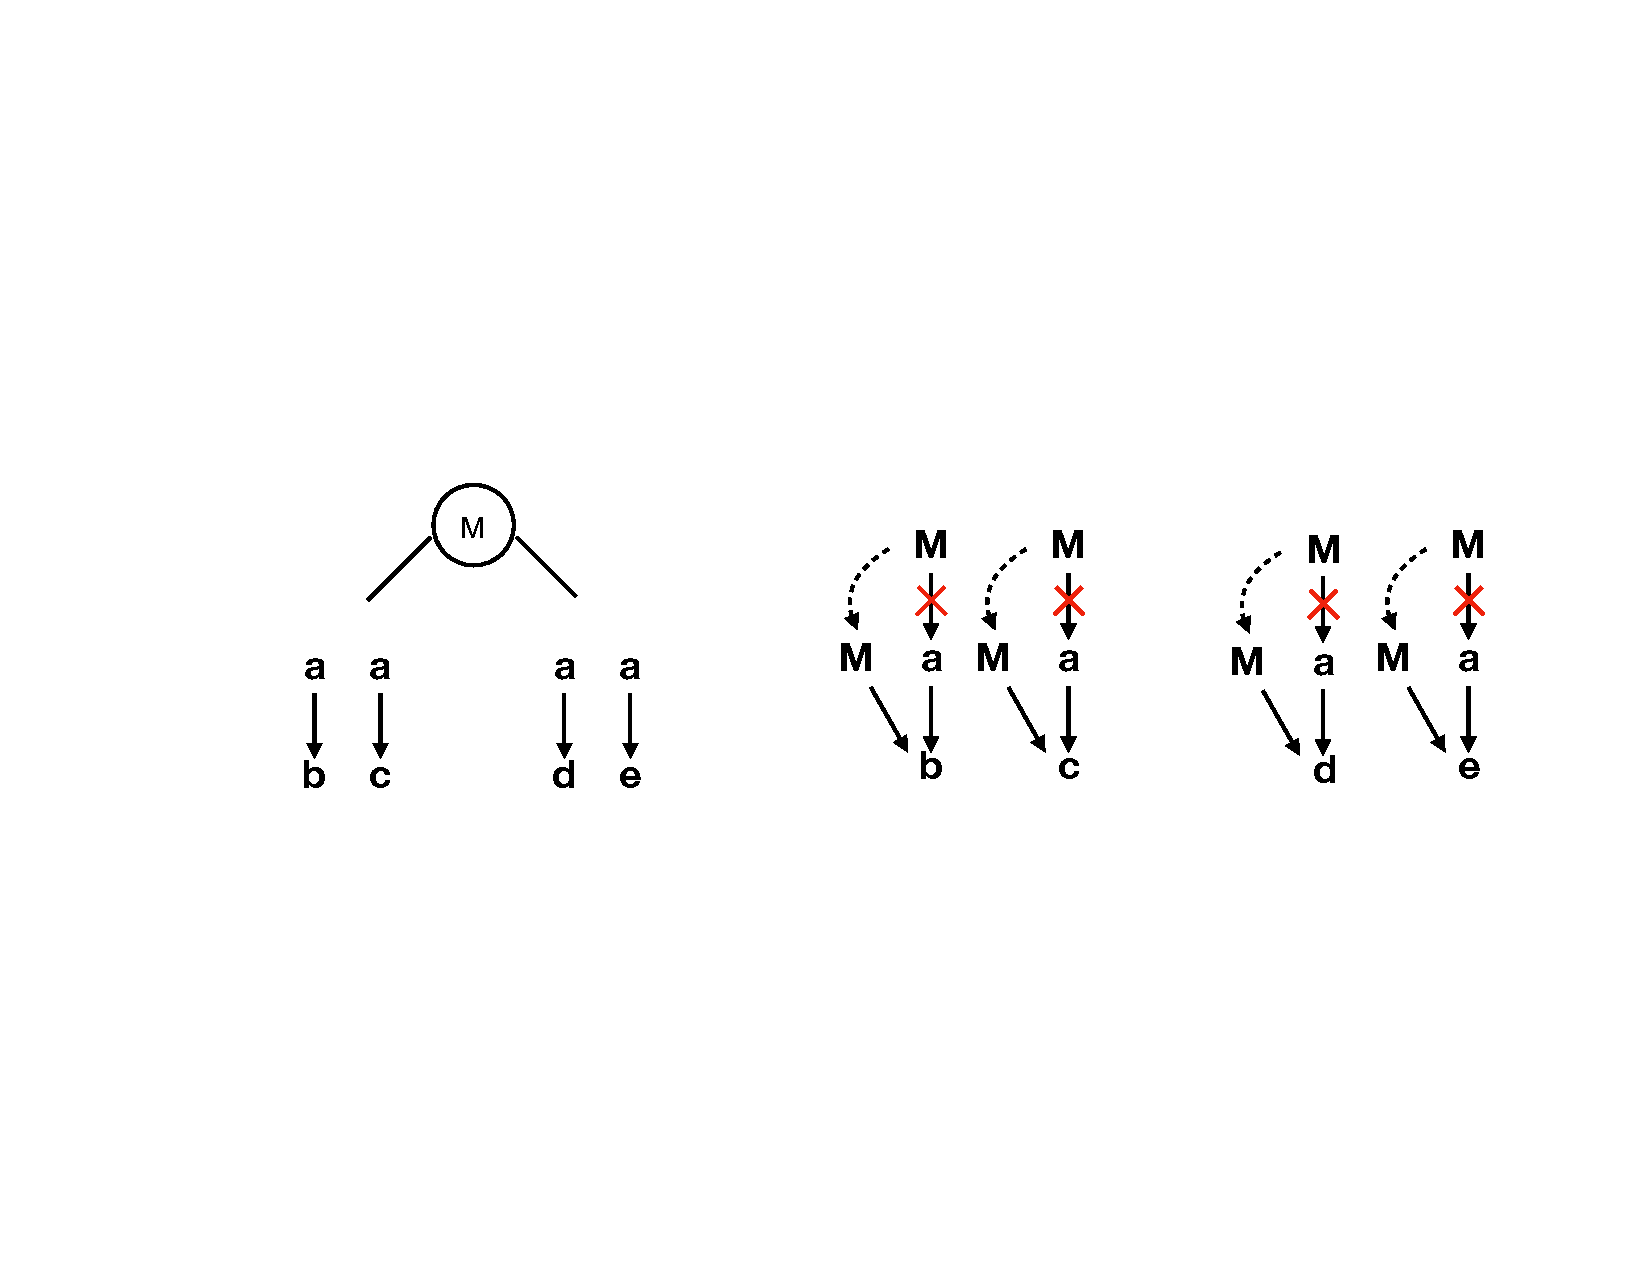
\includegraphics[width=\linewidth]{figures/ss-129.pdf}
\caption{\small Skip the same nodes.}
%\vspace{-1mm}
\label{fig:skip}
\end{figure}

\subsection{数据平面配置生成}

\para{删除DG中冗余节点}:完成路径计算后,DG中的每一个叶子节点都有一个具体路径。基于数据包转发模型,网络中所有交换机上的DG都相同。不难发现,如果一个交换机不属于一条路径,则相应的叶子节点应该被删除(同时删除出度为零的中间节点)。同时,通过将路径转化为交换机的下一跳,我们可以进一步删除冗余节点。考虑防火墙的例子,当路径转化为下一跳后,我们发现中间盒节点的两个叶子节点相同,即网络中的交换机$a$。这意味着该中间盒处理节点对于网关$gw$没有任何意义,因为不管处理结果如何,其下一跳不变。因此,我们可以删除该节点并替换为下一跳为$a$的叶子节点。图~\ref{fig:rv}给出了该过程。


%\para{Remove redundant nodes of DG}: After the path computation, there are concrete paths for all the leaf nodes in DG. We follow the packet forwarding model described previously that all the switches in the network have the same DG. It is easy to observe that if a switch does not belong to a path, then the corresponding leaf node of the path can be removed (and then the no-out-edge internal nodes). Also, by converting the path in a leaf node to the next hop in the network, we may still remove redundant nodes. Still consider the firewall example. After we convert the paths to next hops, we find that the two leaf nodes of the middlebox node are the same, \ie, switch $a$ in the network. This means the middlebox-operation node has no meaning for the gateway $gw$ since whatever the result of the node is, the next hop does not change. Therefore, we can remove the node and replace with the leaf node with the next hop $a$. Fig.~\ref{fig:rv} illustrates the process. 

对于交换机,基于更新后的DG,并根据多流表pipeline的架构,其流表的结构以及流表内容可以简单地生成。其中一个中间盒处理节点可以看作一对状态表和匹配表。对于中间盒,如果它是无状态中间盒,则对于其数据平面,只需要配置交换机到中间盒的隧道;如果它是有状态中间盒,由于它处在计算出的转发路径之中,因此可以看作是有状态交换机,同时可以将结果嵌入到数据包中。当一个数据包在一个交换机的DG中遇到一个有状态中间盒节点,并且该节点无法被叶子节点替换时,该节点下的任意下一跳都是可以接受并正确的,因为它最终会到达相应的中间盒,并且从该交换机到中间盒的任意一条路径一定满足路径约束。

%Then, for the switch side, based on the updated DG, it can generate tables and flow rules easily with the multi-table pipeline structure. Note that a middlebox-operation node can be viewed as a state table following a match table. As for the middlebox side, if it is a stateless middlebox, then for the datapath it only needs to care about is switch-middlebox tunnels which also can be easily generated. For the stateful middleboxes, as they belong to computed paths, they can be viewed as switch nodes with stateful functions that can embed the results to the packets. When a packet meets a stateful middlebox node in DG of a switch, and the node cannot be replaced with a leaf node, then any next hop under the node is acceptable since it must eventually arrive at the middlebox and any path from the switch to the middlebox must follow the path constraints.

\begin{figure}[!htbp]
%\vspace{-2mm}
\centering
      \centering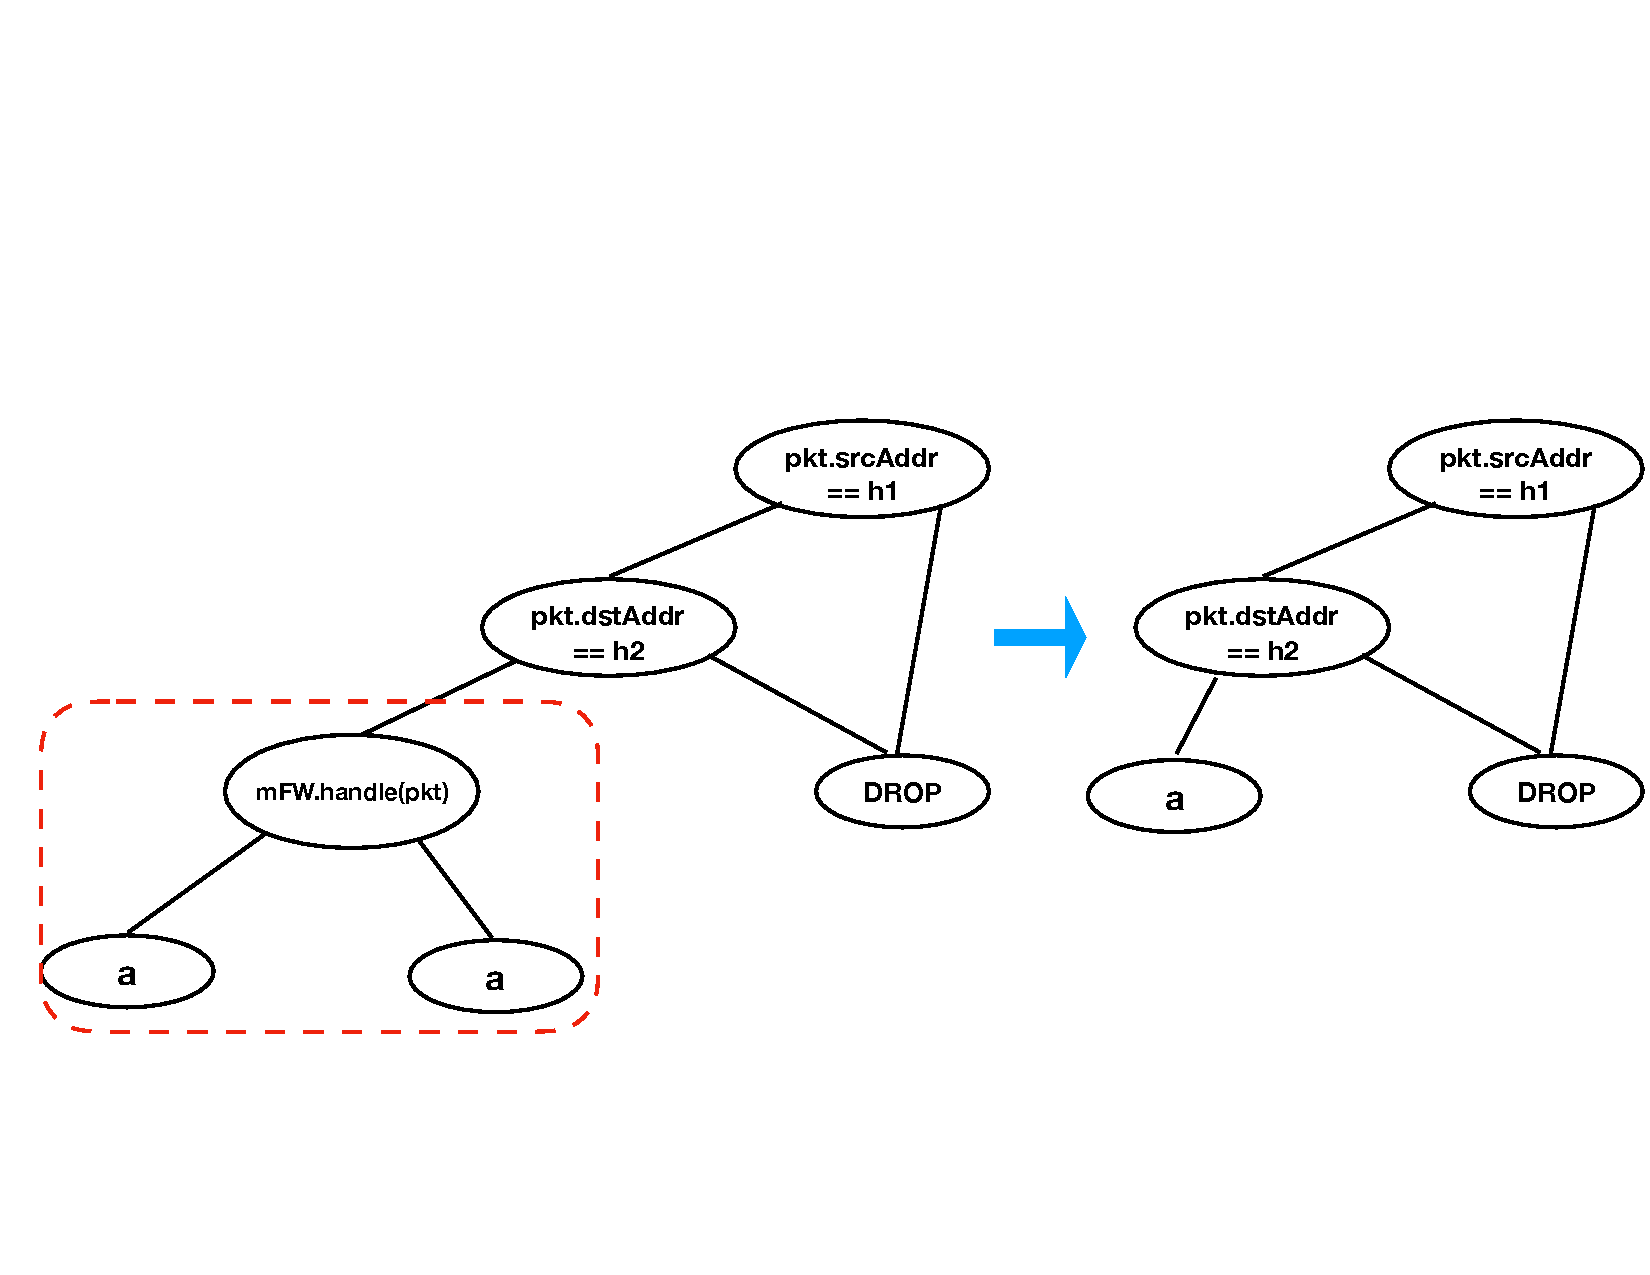
\includegraphics[width=\linewidth]{figures/ss-130.pdf}
\caption{删除冗余中间盒节点。}
%\vspace{-2mm}
\label{fig:rv}
\end{figure}

\para{消息次序}:当无状态中间盒共享本地状态(即更新状态)到交换机时要考虑消息的次序问题。对于目标的交换机,需要保证更新消息要比数据包提前到达。例如,在防火墙例子中,只有第二步完成后,第三步才可以执行。因此一个简单的做法是让数据包携带更新消息。而与有状态中间盒的数据包携带状态不同的是,该消息可以添加或修改相应中间盒处理节点的状态表。

%\para{Order of messages}: The next issue is how a stateless middlebox share local states (\ie, update states) in other switches. It needs to guarantee that for any targeting switch, the update message should arrive earlier than the packet. For example, in the firewall example, only the step 2 is finished, step 3 can be executed. Then a simple solution can be making the packet carry the update message. Different with the state carrying for stateful middleboxes, this message can install/modify rules in the state table of the corresponding middlebox-operation node.

\section{实验评估}

本节中,我们先分别从时延和吞吐量两个方面验证Dandelion的优势。然后给出基准点约束计算部分的评估测试。实验环境是3.5 GHz Intel i7处理器、16 GB内存、Mac OSX 10.13系统。

%In this section, we will first demonstrate the benefits of \concept{} from two aspects: latency and total throughput, and then give the evaluation for the waypoints constraints computation part. All evaluations are run on an 3.5 GHz Intel i7 processor with 16 GB of RAM running Mac OSX 10.13.

\para{实验方法}:首先我们随机生成一个具有25个节点和50条边的网络。对于网络中的每一个边,我们设置两个随机值,分别代表时延(5 - 10 ms)和带宽(5 - 10 Mbps)。为了模拟数据流,我们在网络中随机地选择两个点分别作为数据流的源节点和目的节点。同时一个数据流可以有一个网络中的节点序列(除了本身的源和目的节点)作为其数据包处理需要的有序的中间盒节点。对于中间盒节点的选择,我们添加如下约束:中间盒节点的邻居节点数量为2。这是因为普遍的中间盒没有路由功能,对于收到的数据包,其转发接口只有一个。作为Dandelion的对比,我们考虑一个传统的方法,即路径的计算对于中间盒不区分有状态或无状态。因此,该方法需要保证计算出的路径必需按正确顺序经过所有中间盒。而对于Dandelion中的路径计算,我们在这些中间盒中随机选择一些作为有状态中间盒,则其余为无状态中间盒。

%\para{Methodology}: First we generate a random topology with 25 nodes and 50 edges. For every edge, we set two random values as its latency (5 - 10 ms) and bandwidth (5 - 10 Mbps). To model a flow in the topology, we randomly choose two nodes from the topology as the source and destination nodes of the flow. And a flow can have a sequence of nodes (other than its source and destination nodes) in the topology as its required ordered middleboxes for packet processing. (We add a constraint to the selection for these middlebox nodes that the number of neighbors of a middlebox node must equal to two as typically a middlebox does not have route selection capability, \ie, for any packet, it only has one output interface.) As a comparison of \concept{}, the traditional approach does not distinguish whether a middlebox is stateful or stateless. Therefore, when computing a path for a flow in the tradition way (\ie, do not apply \concept{}), it requires the path must pass through all the middleboxes in a correct order. And when computing a path for a flow in the \concept{} approach, we random choose a subset of its required middlebox nodes as stateful middleboxes since for \concept{} approach, stateful and stateless middleboxes are handled in different ways.

\para{时延}:为了验证对于时延的优势,我们考虑单个数据流并变化其需要的中间盒数量。目标为计算出具有最低时延的路径。然后,我们在应用Dandelion和不应用Dandelion之间比较时延结果。

%\para{Latency}: To show the benefits for the latency aspect, we consider a single flow and differentiate its number of required middleboxes. And the target is to find the optimal path to minimize the latency for the flow. Then, we compare the results (\ie, the minimal latency) between applying \concept{} and not.

\para{吞吐量}:为了验证对于吞吐量的优势,我们考虑多个具有相同的中间盒需求的数据流并变化中间盒的数量。目标为计算出具有最大吞吐量的路径。然后,我们在应用Dandelion和不应用Dandelion之间比较吞吐量结果。

%\para{Total throughput}: To show the benefits for the total throughput aspect, we consider multiple flows and all flows have the same required middleboxes. We also differentiate the number of middleboxes. And the target is to find optimal paths that have maximum total throughput. Then, we compare the results (\ie, the maximum total throughput) between applying \concept{} and not.

\para{执行时间}:为了评估Dandelion的性能,我们分别计算两种方法(即应用Dandelion和不应用Dandelion)中在计算最大吞吐量场景时的路径计算部分执行时间。

%\para{Execution time}: To evaluate the performance of \concept{}, we compare the execution time of the path computation to maximize total throughput for both approaches (\ie, applying \concept{} and not).

\para{基准点约束计算}:为了验证基准点约束计算的优势,我们首先设置网络中的一组节点作为一个数据流的基准点序列。然后,我们考虑低时延作为系统目标并比较应用基准点约束计算和不应用(即过度约束)的结果。在过度约束中,在经过基准点前,需要经过所有的要求的中间盒节点。

%\para{Waypoints constraints computation}: To show the benefits of the waypoints constraints computation, we set a sequence of nodes in the topology as a flow's waypoints constraint. Then, we consider the minimal latency as system's objective and compare the results between applying the waypoints constraints computation and not (\ie, leading to excessive constraints). In the excessive constraints, all the middlebox nodes should be passed through before flow's waypoints.

\para{结果}:如图~\ref{fig:eval12}(a)所示,通过应用Dandelion,时延可以被有效地降低。其中$F$表示数据流的数量;$M$表示要求的中间盒的数量;$S$表示有状态中间盒的数量。由于对于一个数据流的最小时延计算独立于其他数据流,因此实验只考虑一个数据流的场景。从结果中可以看出,在不应用Dandelion情况下,随着无状态中间盒数量的增加,时延会变大;而应用Dandelion情况下,时延只在有状态中间盒数量增加是变大。

%\para{Results}: The results in Fig.~\ref{fig:eval12}(a) demonstrate that by using \concept{}, the latency can be reduced. Specifically, $F$ specifies the number of flows; $M$ specifies the number of required middleboxes for flows; $S$ specifies the number of stateful middleboxes for flows. As minimizing latency for a flow does not affect the results of other flows, the experiment only considers one flow scenario. From the results, we can see that without \concept{}, the latency of the flow grows up when the number of stateless middleboxes increases but if \concept{} is applied, the latency grows up only when the number of stateful middleboxes increases.

如图~\ref{fig:eval12}(b)所示,通过应用Dandelion,吞吐量可以有效地提高。当有五个数据流和三个中间盒时,应用Dandelion的吞吐量是不应用Dandelion的近三倍。

%The results in Fig.~\ref{fig:eval12}(b) demonstrate that by using \concept{}, the total throughput can be increased. Specifically, when there are 5 flows and 3 middleboxes, the total throughput with \concept{} is around 3 times compared with that without \concept{}.

\begin{figure}[!htbp]
%\vspace{-2mm}
\centering
\subfigure[不同场景下的时延。]{
      \label{fig:eval1} 
      \centering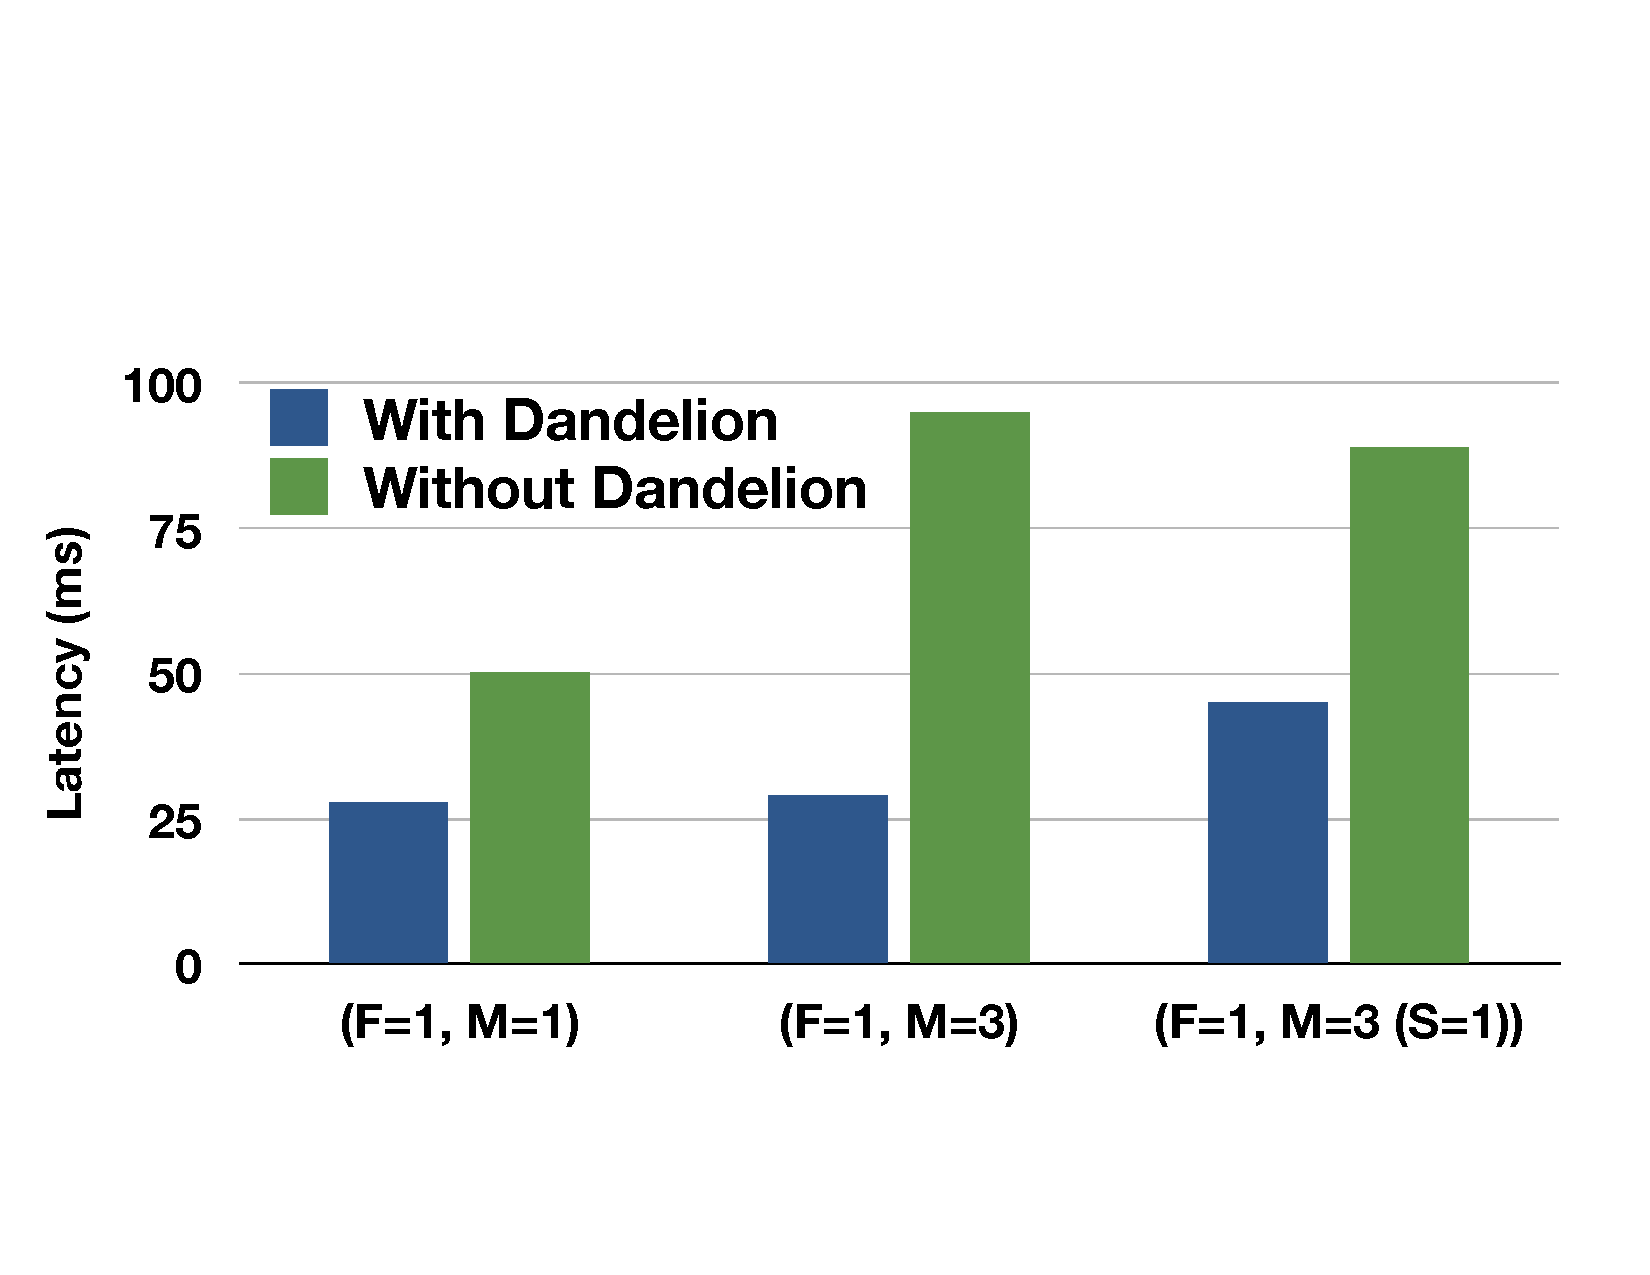
\includegraphics[width=\linewidth]{figures/ss-eval1.pdf}}
%\hspace{0.03\linewidth}
\subfigure[不同场景下的吞吐量。]{
     \label{fig:eval2} 
      \centering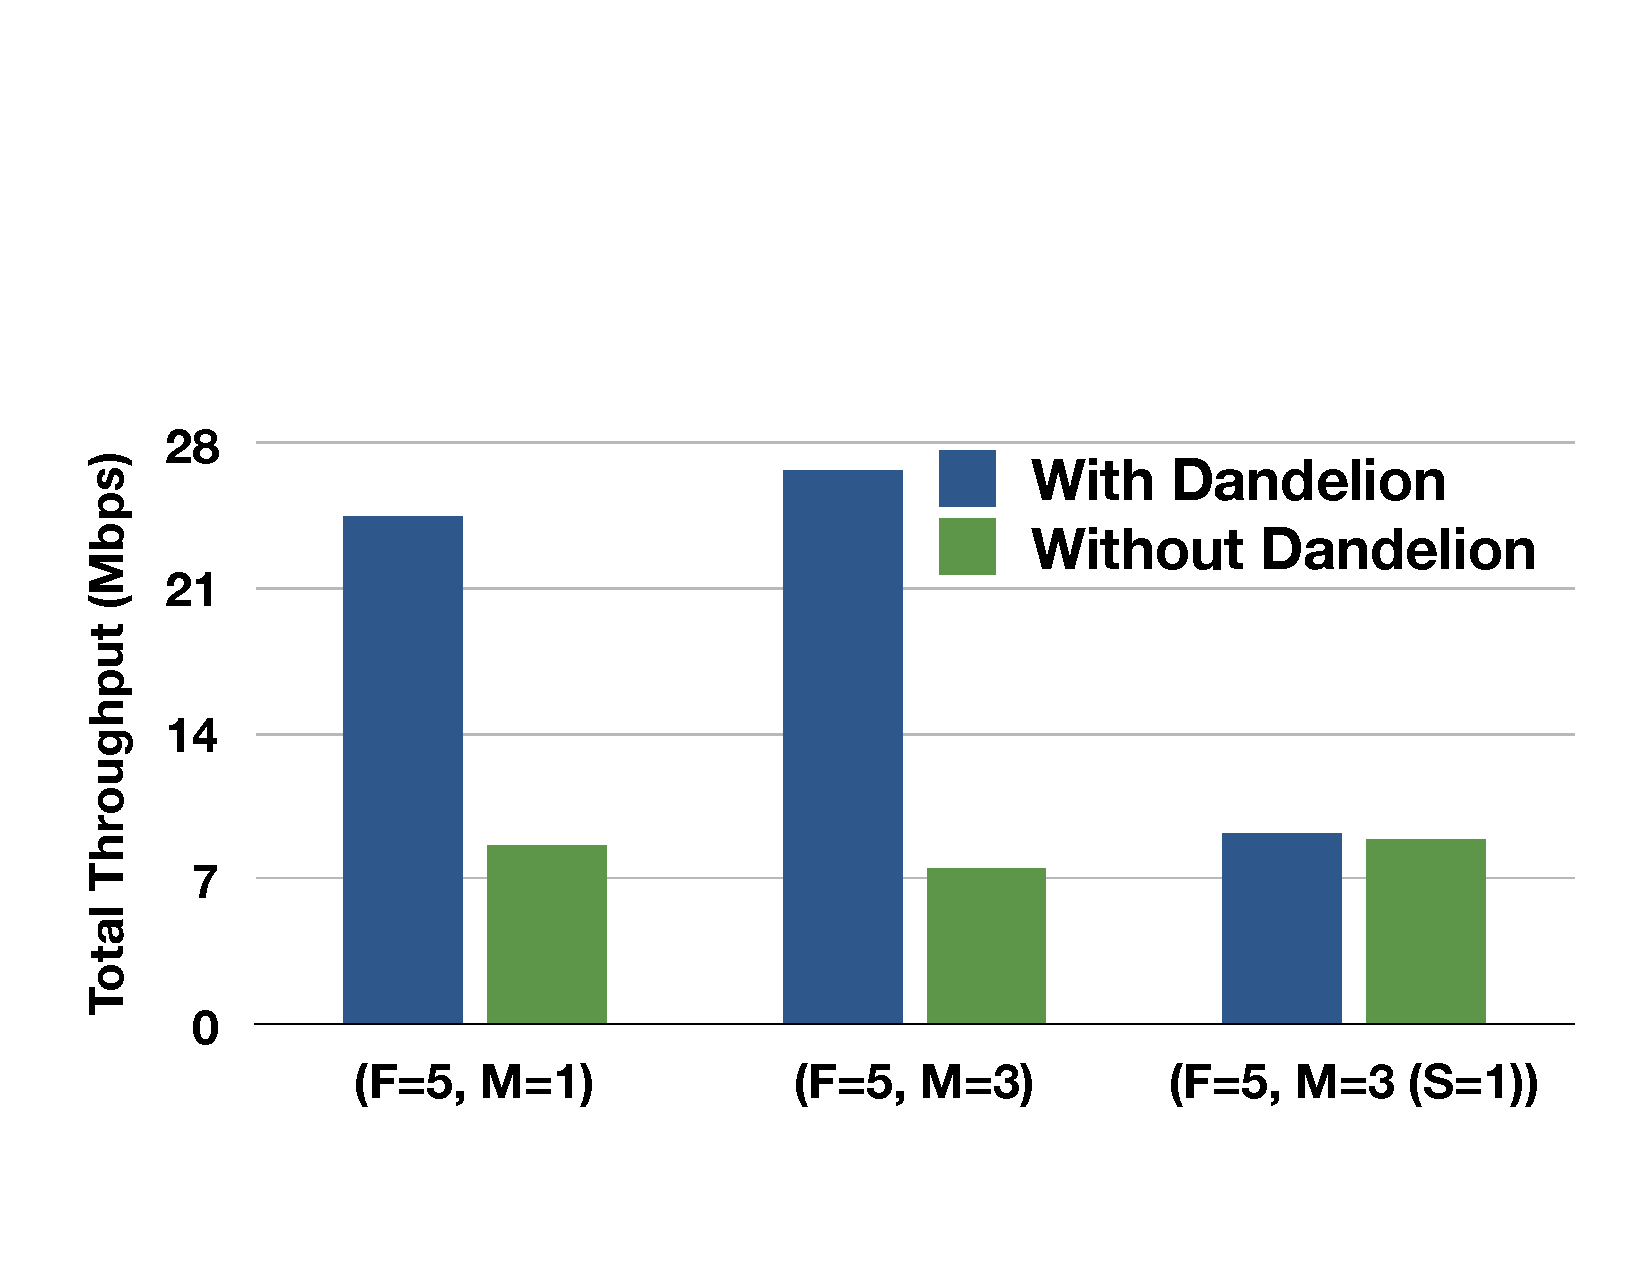
\includegraphics[width=\linewidth]{figures/ss-eval2.pdf}}
\caption{Dandelion对于时延和吞吐量的优势。}
%\vspace{-2mm}
\label{fig:eval12}
\end{figure}




%\begin{figure}[!htbp]
%%\vspace{-2mm}
%\centering
%\begin{subfigure}{0.8\linewidth}
%      \centering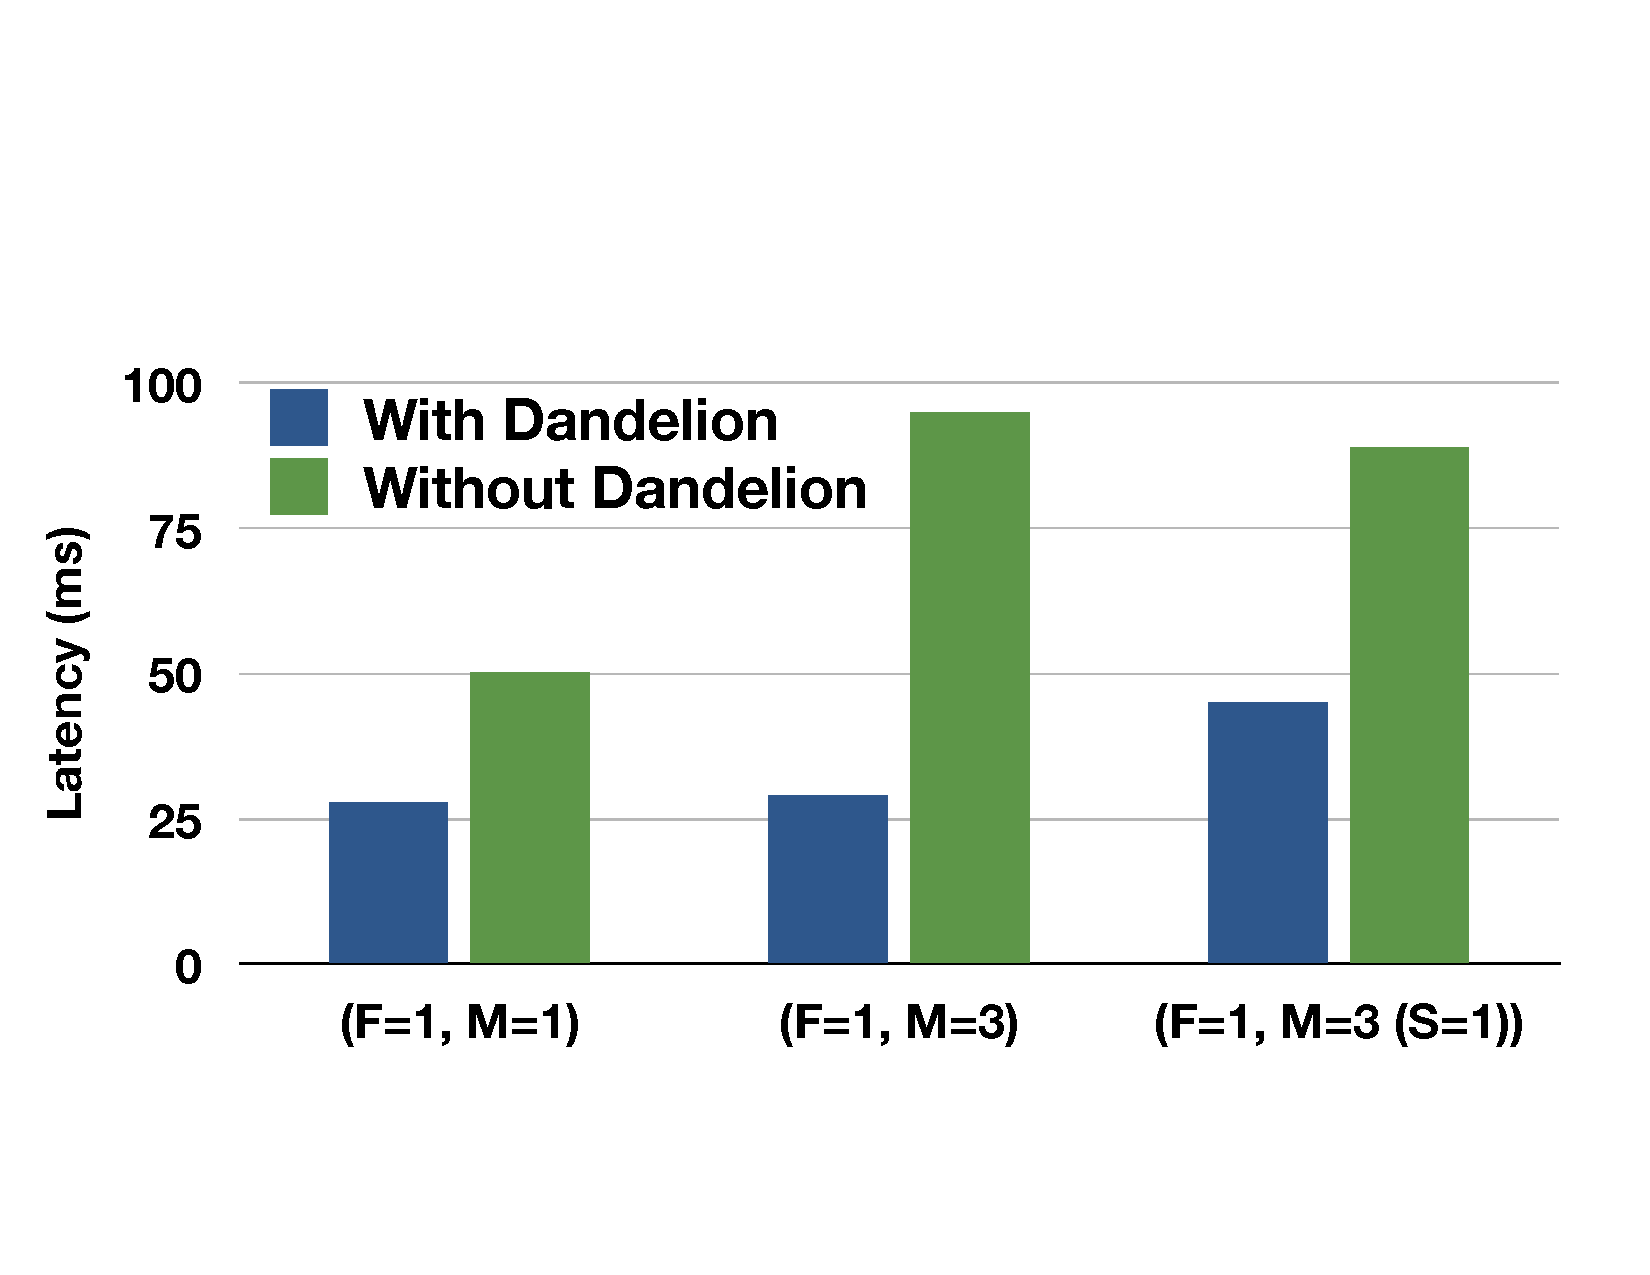
\includegraphics[width=\linewidth]{figures/ss-eval1.pdf}
%\end{subfigure}
%\hspace{0.03\linewidth}
%%\vspace{-2mm}
%%\caption{\footnotesize{The CDF of job latency local and remote jobs.}}
%\caption{\small The latency for different scenarios.}
%%\vspace{-2mm}
%\label{fig:eval1}
%\end{figure}




%\begin{figure}[!htbp]
%%\vspace{-2mm}
%\centering
%\begin{subfigure}{0.8\linewidth}
%      \centering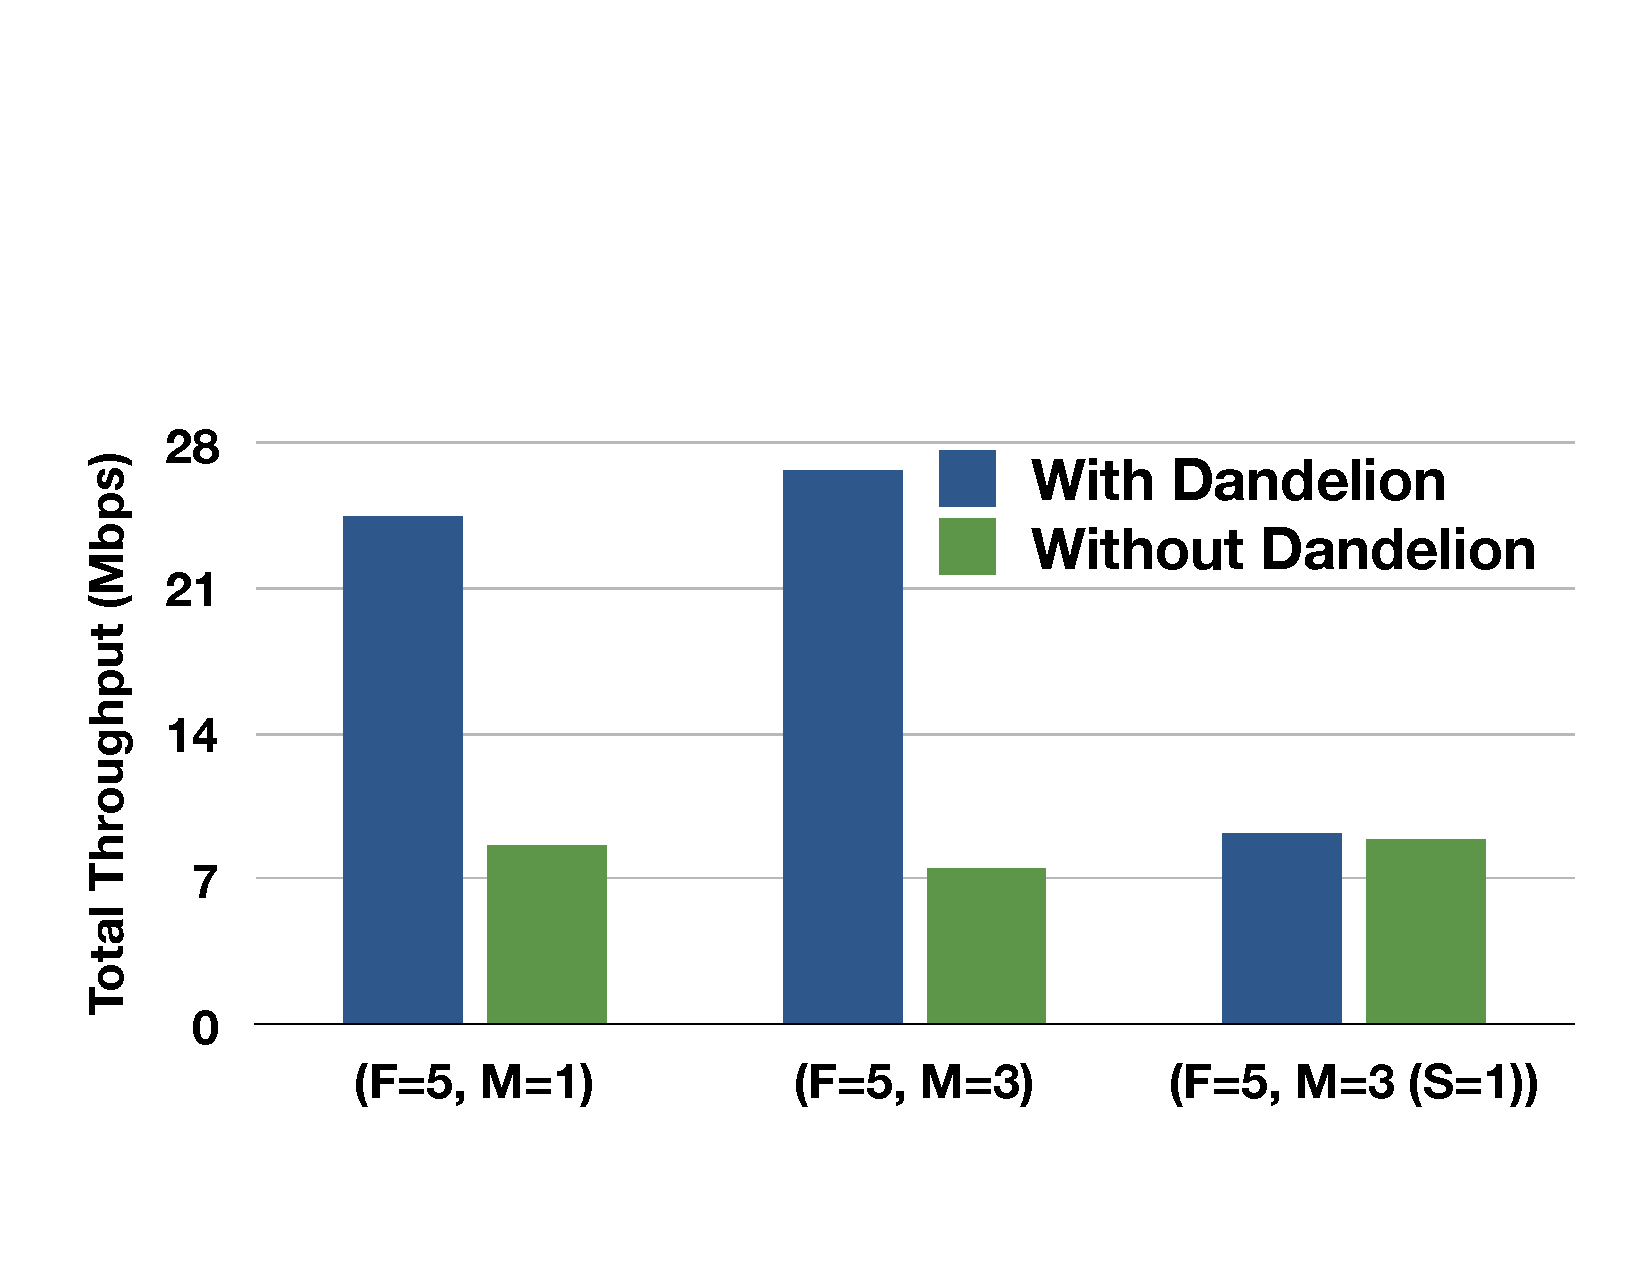
\includegraphics[width=\linewidth]{figures/ss-eval2.pdf}
%\end{subfigure}
%\hspace{0.03\linewidth}
%%\vspace{-2mm}
%%\caption{\footnotesize{The CDF of job latency local and remote jobs.}}
%\caption{\small The total throughput for different scenarios.}
%%\vspace{-2mm}
%\label{fig:eval2}
%\end{figure}

表格~\ref{table:eval1}显示的是在计算最大吞吐量时路径计算部分的执行时间。由于在应用Dandelion情况下,约束的数量少于不应用Dandelion情况,因此执行时间也会相应的降低(当F=5,M=3时,从10.8秒降为1.4秒)

%The results in Table~\ref{table:eval1} show the execution time of the path computation part to maximize total throughput. Since with \concept{}, the number of constraints is smaller than that without \concept{}, the execution time is also reduced (from 10.8 to 1.4 seconds when F=5 and M=3). 


\begin{table}[]
\footnotesize
\begin{tabular}{|l|l|l|l|}
\hline
             & \footnotesize(F=5, M=1) & \footnotesize (F=5, M=3) & \footnotesize (F=5, M=3 (S=1)) \\ \hline
With Dandelion    & 1.3 (s)    & 1.4 (s)    & 4.2 (s)          \\ \hline
Without Dandelion & 4.5 (s)    & 10.8 (s)   & 11.5 (s)         \\ \hline
\end{tabular}
\caption{\small The execution time of path computation to maximize total throughput for different scenarios.}
\label{table:eval1}
\end{table}

图~\ref{fig:eval34}给出的是有正确约束(即通过应用基准点约束计算)和有过度约束的时延结果。其中图~\ref{fig:eval34}(a)对应的是只有一个基准点,而图~\ref{fig:eval34}(b)对应的是三个基准点。从结果中我们可以看出,过度约束会增加时延,其理由是非最优的路径计算。而随着基准点的数量增加,有过度约束的时延也会变大。


%Fig.~\ref{fig:eval34} shows the latency with correct constraints (\ie, by
%applying waypoints constraints computation) and with excessive constraints.
%Specifically, the results in Fig.~\ref{fig:eval34}(a) consider that the
%waypoints only have one node while Fig.~\ref{fig:eval34}(b) are for three nodes.
%From the results, we can see the excessive constraints increase the latency,
%\ie, lead to non-optimal path computation result. As the number of nodes
%increases in the waypoints constraint, the latency with excessive constraints becomes larger.

\begin{figure}[!htbp]
%\vspace{-2mm}
\centering
\subfigure[ 基准点约束中有一个节点。]{
      \label{fig:eval3}
      \centering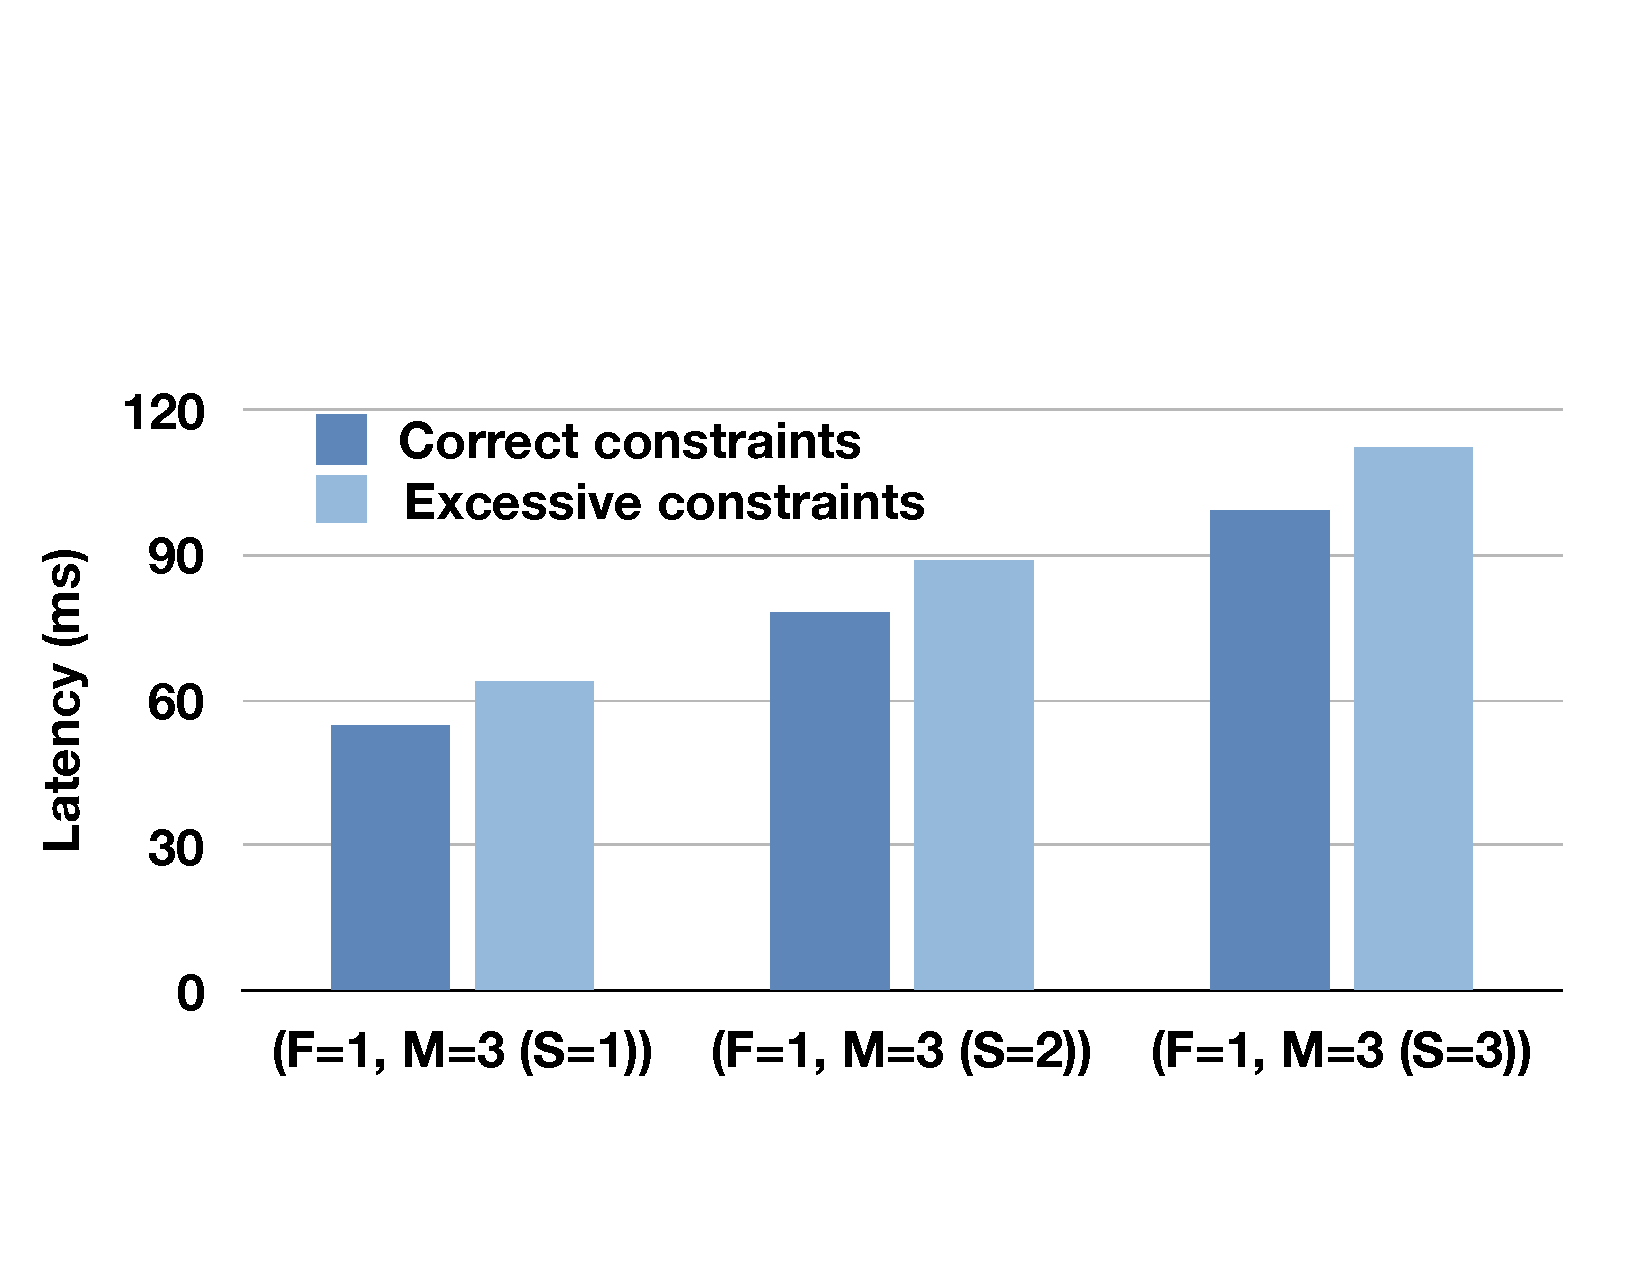
\includegraphics[width=\linewidth]{figures/ss-eval3.pdf}}
%\hspace{0.03\linewidth}
\subfigure[ 基准点约束中有三个节点。]{
      \label{fig:eval4} 
      \centering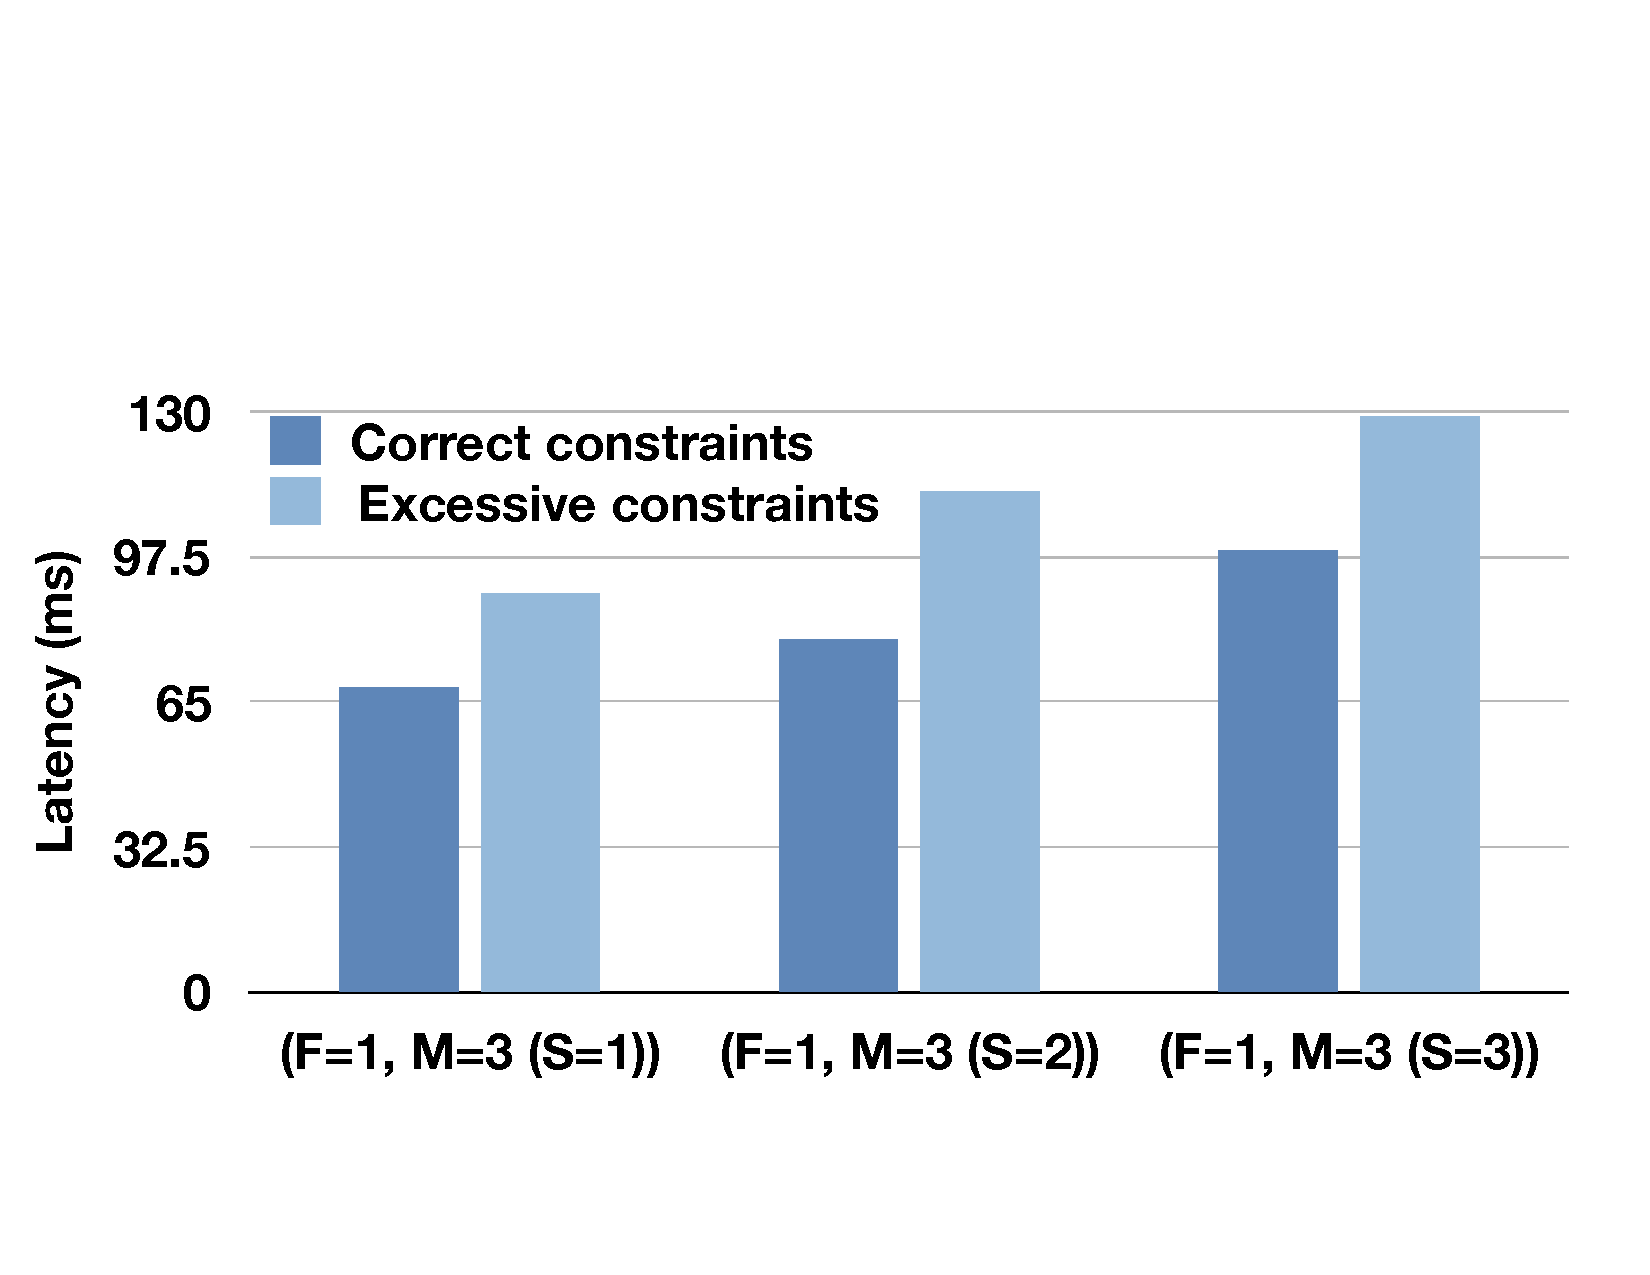
\includegraphics[width=\linewidth]{figures/ss-eval4.pdf}}
\caption{不同基准点约束下的时延。}
%\vspace{-2mm}
\label{fig:eval34}
\end{figure}


\section{本章小结}

本章针对SDC网络设计高级编程系统Dandelion,并基于共享本地状态的方法,优化系统性能。实验表明在某些场景下吞吐量可以实现近三倍的提高。





 
\end{document}